\chapter{Bivariate analyse}
\label{ch:analyse2var}

In de vorige hoofdstukken hebben we telkens één variabele tegelijkertijd onderzocht. In dit hoofdstuk bestuderen we \emph{verbanden}\index{verband} (ook: \emph{samenhang}\index{samenhang} of \emph{associatie}\index{associatie}) tussen variabelen. We spreken van een verband tussen twee variabelen wanneer de waarde van de ene variabele op een systematische manier verandert ten opzichte van de waarde van de andere. Anders gezegd, wanneer we tot op zekere hoogte een voorspelling kunnen doen over de waarde van een variabele aan de hand van de waarde van een andere.

\section{Leerdoelen}
\label{sec:analyse2var-leerdoelen}

Na dit hoofdstuk moet je in staat zijn om:

\begin{itemize}
  \item De volgende begrippen uit dit hoofdstuk uit te leggen:
  \begin{itemize}
    \item afhankelijke variabele, onafhankelijke variabele;
    \item een verband (samenhang, associatie) tussen twee variabelen, stijgend/dalend verband, lineair verband;
  \end{itemize}
  \item Voor de in dit hoofstuk besproken combinaties van meetniveaus geschikte analysetechnieken te benoemen;
  \item Voor een combinatie van twee kwalitatieve variabelen:
  \begin{itemize}
    \item Een kruistabel op te stellen en de regel van Cochran toe te passen;
    \item De $\chi^2$-statistiek te berekenen;
    \item De $\chi^2$-toets uit te voeren (voor associatie en goodness-of-fit);
    \item Gestandaardiseerde residuën te berekenen en te interpreteren;
    \item Cramér's V te berekenen en de waarde te interpreteren
  \end{itemize}
  \item Voor een combinatie van een kwalitatieve onafhankelijke en kwantitatieve afhankelijke variabele:
  \begin{itemize}
    \item De correcte variant van de $t$-toets voor twee steekproeven (gepaard, onafhankelijk) toe te passen;
    \item De effectgrootte (Cohen's $d$) te berekenen en de waarde te interpreteren;
  \end{itemize}
  \item Voor een combinatie van twee kwantitatieve variabelen:
  \begin{itemize}
    \item het functievoorschrift van de regressierechte te bepalen en die te tekenen;
    \item de covariantie, correlatiecoëfficiënt en determinatiecoëfficiënt te berekenen en de waarde ervan met de correcte verwoordingen te interpreteren;
  \end{itemize}
  \item Voor de in dit hoofstuk besproken combinaties van meetniveaus geschikte visualisatietechnieken te benoemen en toe te passen;
  \item Een gegeven grafiek met twee variabelen te interpreteren, o.a.~het grafiektype benoemen, afleiden of er een verband bestaat, welk soort verband en de mate van associatie (zwak, matig, sterk).
  \item Aan de hand van een situatie kunnen uitleggen dat een verband niet noodzakelijk een noodzakelijk verband inhoudt, en waarom;
\end{itemize}

\section{Inleiding}
\label{sec:analyse2var-inleiding}

Wanneer we een verband beschrijven tussen variabelen, onderscheiden we:

\begin{itemize}
  \item De \emph{afhankelijke variabele}\index{variabele!afhankelijke}, waarover we een voorspelling willen doen;
  \item De \emph{onafhankelijke variabele}\index{variabele!onafhankelijke}, op basis van dewelke we de voorspelling doen.
\end{itemize}

Dus als de onafhankelijke variabele op een bepaalde manier verandert, verwachten we dat de waarde van de afhankelijke variabele op een voorspelbare manier mee verandert.

\begin{example}
  Een voorbeeld waarbij verbanden kunnen gevonden worden tussen variabelen vind je bij Ant Colony Optimization (ACO). Dit is een techniek die gebruikt wordt in verschillende computationele problemen. Men baseert zich hier op hoe mieren voedsel zoeken en  vinden en dat communiceren aan de groep. Mieren verspreiden feromonen als ze op pad gaan op zoek naar eten. Hoe langer het pad, hoe minder feromonen het pad zal bevatten, hoe korter het pad, hoe groter de kans dat er een grote concentratie aan feromonen te vinden is. Mieren worden aangetrokken door deze feromonen en zullen dus proberen de meest bewandelde paden te gebruiken om naar een bepaalde voedselbron te gaan. Nu kan je onderzoeken of de tijd voor het vinden van een pad, afhangt van een aantal variabelen:

  \begin{itemize}
    \item De mate waarin feromonen verspreid worden
    \item De mate waarin een feromoon verdwijnt
    \item Het aantal obstakels tussen het nest en de voedselbron
    \item De vorm van de obstakels tussen nest en voedselbron (vinden ze sneller het pad indien er geen hoeken aan de obstakels zijn bv.)
  \end{itemize}
\end{example}

Voor het onderzoeken of er een verband bestaat tussen twee variabelen bestaan er verschillende analyse- en visualisatietechnieken die afhangen van het meetniveau. Tabel~\ref{tab:analyse2var} geeft een overzicht van geschikte analysetechnieken die in deze cursus besproken worden en Tabel~\ref{tab:visualisatie2var} van geschikte grafiektypes.

Merk trouwens op dat er nog veel meer analysetechnieken bestaan die niet in deze cursus besproken worden! Hier vind je enkel een topje van de ijsberg\ldots Als je in je latere carrière nood hebt aan statistische technieken (en de auteurs van deze cursus zijn optimistisch dat dit ook effectief ooit eens zal gebeuren), kijk je best na of er betere technieken bestaan voor het beantwoorden van jouw specifieke onderzoeksvraag.

\begin{table}
  \begin{tabular}{llll}
    \toprule
    \textbf{Onafhankelijke} & \textbf{Afhankelijke} & \textbf{Toets}                & \textbf{Metriek}      \\
    \midrule
    Kwalitatief             & Kwalitatief           & $\chi^2$-toets                & Cramér's $V$          \\
    Kwalitatief             & Kwantitatief          & $t$-toets voor 2 steekproeven & Cohen's $d$           \\
    Kwantitatief            & Kwantitatief          & ---                           & Regressie, correlatie \\
    \bottomrule
  \end{tabular}
  \caption{Overzicht van analysetechnieken voor het verband tussen twee variabelen. De tabel geeft telkens enerzijds geschikte statistische toetsen en anderzijds metrieken die de mate van het verband uitdrukken.}
  \label{tab:analyse2var}
\end{table}

\begin{table}
  \begin{tabular}{lll}
  	\toprule
  	\textbf{Onafhankelijke} & \textbf{Afhankelijke} & \textbf{Grafiektype}                                  \\
  	\midrule
  	Kwalitatief             & Kwalitatief           & Mozaïekdiagram, rependiagram, geclusterd staafdiagram \\
  	Kwalitatief             & Kwantitatief          & Boxplot, staafdiagram met error bars                  \\
  	Kwantitatief            & Kwantitatief          & Spreidingsdiagram, regressierechte                    \\
  	\bottomrule
  \end{tabular}
  \caption{Overzicht van visualisatietechnieken voor het verband tussen twee variabelen.}
  \label{tab:visualisatie2var}
\end{table}

\section{Kwalitatief--kwalitatief}
\label{sec:kwalitatief-kwalitatief}

In deze sectie bekijken we methoden om na te gaan of er een verband bestaat tussen twee kwalitatieve variabelen. Al deze methoden zijn gebaseerd op een samenvattende tabel van frequenties van de twee variabelen, de kruistabel (zie Sectie~\ref{ssec:kruistabellen}). Daaruit wordt een statistiek berekend die uitdrukt hoe groot de verschillen zijn tussen de twee variabelen, de zogenaamde ``Chi-kwadraat'', notatie $\chi^2$\footnote{Chi, $\chi$ is een letter uit het Griekse alfabet.} (zie Sectie~\ref{ssec:chi-kwadraat}). Met de $\chi^2$-toets (zie Sectie~\ref{ssec:onafhankelijkheidstoets} en~\ref{ssec:aanpassingstoets}) kan je nagaan of de waarde van $\chi^2$ al dan niet aangeeft of er een verband bestaat tussen twee variabelen. Er bestaat ook een metriek, Cramér's $V$ (zie Sectie~\ref{ssec:cramers-v}), die de waarde van $\chi^2$ herleidt tot een getal tussen 0 en 1 waaruit de sterkte van het verband valt af te leiden.

\subsection{Kruistabellen}
\label{ssec:kruistabellen}

\begin{definition}[Kruistabel]
  In een kruistabel\index{kruistabel} (Eng.: \emph{contingency table} of \emph{cross table}; zie bv.~Figuur~\ref{tab:kruistabel0}) worden de frequenties van twee variabelen samengevat.
  
  Elke cel van de laatste kolom bevat de som van de overeenkomstige rij en elke cel van de laatste rij bevat de som van de overeenkomstige kolom. Dit worden de \emph{marginale totalen}\index{totaal!marginaal}\index{marginaal totaal} genoemd.
\end{definition}

\begin{table} \centering
  \begin{tabular}{@{}rrrr}
    \toprule
                & Vrouw & Man & Totaal \\
    \midrule
           Goed &     9 &   8 &     17 \\
      Voldoende &     8 &  10 &     18 \\
    Onvoldoende &     5 &   5 &     10 \\
         Slecht &     0 &   4 &      4 \\
         Totaal &    22 &  27 &     49 \\
    \bottomrule
  \end{tabular}
  \caption{Een kruistabel voor de waardering door mannen en vrouwen van een bepaald assortiment producten.}
  \label{tab:kruistabel0}
\end{table}

Hoe kunnen we nu zien in een kruistabel of er een verband bestaat tussen twee variabelen? Bekijk de kruistabel in Tabel~\ref{tab:kruistabel0}. Die geeft de resultaten weer van een bevraging waar 49 mensen (22 vrouwen en 27 mannen) gevraagd werd om een waardering te geven (goed, voldoende, onvoldoende of slecht). Als er een verband bestaat tussen de twee variabelen, gender (onafhankelijk) en waardering (afhankelijk), dan moeten we zien dat vrouwen en mannen fundamenteel andere waarderingen gegeven hebben. Omgekeerd, als zowel bij de vrouwen als bij de mannen de verhoudingen tussen de verschillende waarderingen (ongeveer) gelijk zijn, dan is er \emph{geen} verband.

In een gewone kruistabel kunnen we geen directe conclusies trekken, aangezien het analyseren of er samenhang bestaat tussen variabelen niet goed gaat op basis van de absolute frequenties. Er zijn immers meer mannen dan vrouwen in de bevraging! Daarom moeten we percenteren, d.w.z.~binnen elke kolom het percentage berekenen hoe vaak elke beoordeling \emph{naar verhouding} voorkomt. De som van alle percentages in een kolom moet dan gelijk zijn aan 100\%. Nog even snel de regel van percenteren:

\begin{itemize}
  \item Om te weten hoeveel procent $x$ is van $y$, deel je $x$ door $y$ en vermenigvuldig je met 100: $p = \frac{x}{y} \times 100$. Bijvoorbeeld: hoeveel procent is 15 van 20? $\frac{15}{20} \times 100 = 75$, dus 75\%.
  \item Om te weten hoeveel $x\%$ is van $y$: $\frac{x \times y}{100}$. Hoeveel is 60\% van 30? $\frac{60 \times 30}{100} = 18$.
\end{itemize}

In Tabel~\ref{tab:kruistabel1} vind je per geslacht de percentages dat elke waardering is voorgekomen in de steekproef. We zien dan bijvoorbeeld dat 41\% van de vrouwen een waardering goed heeft gegeven (want 9 is ongeveer 41\% van 22), tegen dat 30\% van de mannen.

\begin{table} \centering
  \begin{tabular}{@{}rrrrrrr@{}}
  	\toprule
  	            & Vrouw & Man & Totaal & Vrouw \% & Man\% & Totaal \\
  	\midrule
  	       Goed &     9 &   8 &     17 &     41\% &  30\% &   35\% \\
  	  Voldoende &     8 &  10 &     18 &     36\% &  37\% &   37\% \\
  	Onvoldoende &     5 &   5 &     10 &     23\% &  18\% &   20\% \\
  	     Slecht &     0 &   4 &      4 &      0\% &  15\% &    8\% \\
  	     Totaal &    22 &  27 &     49 &    100\% & 100\% &  100\% \\
  	\bottomrule
  \end{tabular}
  \caption{De kruistabel waarbij we de waarden gepercenteerd hebben.}
  \label{tab:kruistabel1}
\end{table}

Nu kunnen we ons de vraag stellen of de waarderingskeuze afhangt van het gender van de respondent. Er zijn verschillen tussen beide kolommen, dus je kan een vermoeden hebben dat dit inderdaad het geval is. Hoe kleiner de verschillen, hoe minder verband er is tussen beide variabelen, hoe groter de verschillen, hoe groter de samenhang.

\subsection{\texorpdfstring{$\chi^{2}$}{chi-kwadraat}}
\label{ssec:chi-kwadraat}

Uit de vorige sectie kunnen we besluiten dat we nood hebben aan een maat die uitdrukt hoe groot het verschil is tussen de verhoudingen in beide kolommen. Een manier om dit uit te drukken wordt de \emph{chi-kwadraat}-statistiek (notatie $\chi^{2}$) genoemd. $\chi^2$ is gelijk aan 0 als er geen verschil is tussen de verhoudingen in de kolommen van een kruistabel, en als er dus ook volstrekt geen samenhang tussen de variabelen is. Als er wel een verschil is, dan is $\chi^2$ een positief getal. Hoe groter de waarde, hoe groter ook de onderlinge verschillen tussen de kolommen en hoe groter dus ook de samenhang.

De procedure om de $\chi^2$ van een kruistabel te berekenen gaat als volgt:

\begin{enumerate}
  \item Stel eerst de kruistabel op samen met marginale totalen (zie tabel \ref{tab:kruistabel0}).
  \item Vervolgens berekenen we voor elke cel de zogenaamde \emph{verwachte frequentie} (notatie $e$ van \emph{expected}). Dat is de absolute frequentie die je in deze cel zou \emph{verwachten} als je veronderstelt dat er helemaal geen samenhang is tussen de variabelen. Deze kan je bereken als volgt:
  
  \begin{equation}
  e = \frac{rijtotaal \times kolomtotaal}{n}
  \end{equation}
  
  met:
  
  \begin{itemize}
    \item $rijtotaal$ totaal van de rij van de betreffende cel
    \item $kolomtotaal$ totaal van de kolom van de betreffende cel
    \item $n$ het aantal observaties
  \end{itemize}
  
  Voor cel$_{1,2}$ (het verwachte aantal mannen dat waardering ``goed'' gegeven heeft) is dit dus $\frac{17 \times 27}{49} \approx 9.37\%$.
  
  \item Dan bereken je het verschil tussen geobserveerde (notatie $o$, \emph{observed}) en verwachte frequentie ($e$). (Zie tabel~\ref{tab:kruistabel2}).
  
  \begin{table} \centering
    \begin{tabular}{@{}rrrrrrr@{}}
    	\toprule
    	            &                       Vrouw &                          Man & Totaal & Vrouw \% &   Man\% &  Totaal \\
    	\midrule
    	       Goed &  $9 -\textcolor{red}{7.63}$ &  $8 - \textcolor{red}{9.36}$ &   $17$ &   $41$\% &  $30$\% &  $35$\% \\
    	  Voldoende & $8 - \textcolor{red}{8.08}$ & $10 - \textcolor{red}{9.91}$ &   $18$ &   $36$\% &  $37$\% &  $37$\% \\
    	Onvoldoende & $5 - \textcolor{red}{4.48}$ &  $5 - \textcolor{red}{5.51}$ &   $10$ &   $23$\% &  $18$\% &  $20$\% \\
    	     Slecht & $0 - \textcolor{red}{1.79}$ &  $4 - \textcolor{red}{2.20}$ &    $4$ &    $0$\% &  $15$\% &   $8$\% \\
    	     Totaal &                        $22$ &                         $27$ &   $49$ &  $100$\% & $100$\% & $100$\% \\
    	\bottomrule
    \end{tabular}
    \caption{De kruistabel waarbij we de verwachte frequentie $e$ (aangeduid in het rood) bepaald hebben voor elke cel en die aftrekken van de geobserveerde frequentie $o$.}
    \label{tab:kruistabel2}
  \end{table}
  
  \item De laatste stap houdt in dat we een berekening gaan maken voor de maat van afwijking voor elke cel. Net zoals bij het berekenen van de variantie van een steekproef (zie Sectie~\ref{sec:varEnSD}) kwadrateren we het verschil zodat het resultaat altijd positief is en zodat grotere afwijkingen zwaarder door zullen wegen in het resultaat.
  
  We gaan ook de afwijking delen door de verwachte frequentie om hen relatief even belangrijk te maken. Bijvoorbeeld: een afwijking van 5 op een verwachte frequentie van 20 is groter dan bv. een afwijking op een verwachte frequentie van 200. Dit geeft dan voor elke cel van de kruistabel de volgende berekening (zie Tabel~\ref{tab:kruistabel3}):
  
  \begin{equation}
  \frac{(o - e)^{2}}{e}
  \end{equation}
  
  \begin{table} \centering
    \begin{tabular}{@{}rrrrrrr@{}}
    	\toprule
    	            &                    Vrouw &                      Man & Totaal & Vrouw \% &   Man\% &  Totaal \\
    	\midrule
    	       Goed & $\textcolor{blue}{0.24}$ & $\textcolor{blue}{0.20}$ &   $17$ &   $41$\% &  $30$\% &  $35$\% \\
    	  Voldoende & $\textcolor{blue}{0.00}$ & $\textcolor{blue}{0.00}$ &   $18$ &   $36$\% &  $37$\% &  $37$\% \\
    	Onvoldoende & $\textcolor{blue}{0.06}$ & $\textcolor{blue}{0.05}$ &   $10$ &   $23$\% &  $18$\% &  $20$\% \\
    	     Slecht & $\textcolor{blue}{1.80}$ & $\textcolor{blue}{1.46}$ &    $4$ &    $0$\% &  $15$\% &   $8$\% \\
    	     Totaal &                     $22$ &                     $27$ &   $49$ &  $100$\% & $100$\% & $100$\% \\
    	\bottomrule
    \end{tabular}
    \caption{De kruistabel waarbij we het verschil gekwadrateerd hebben en gedeeld door de verwachte frequentie, $\frac{(o - e)^2}{e}$ (in het blauw). Merk op dat deze waarden afgerond zijn tot twee cijfers na de komma, en we hier dus een deel van de precisie kwijt spelen.}
    \label{tab:kruistabel3}
  \end{table}
  
  \item Alle resultaten gaan we tenslotte optellen om zo de $\chi^{2}$ te bekomen:
  
  \begin{equation}
  \chi^{2} = \sum \frac{(o - e)^{2}}{e}
  \end{equation}
  
  In het voorbeeld is $\chi^2 \approx 3,8105$.
\end{enumerate}

Nu zegt deze waarde $\chi^2 \approx 3,8105$ op zich nog \emph{steeds} niet zo veel. Onder welke voorwaarden zeggen we dat er al dan niet een verband is tussen beide variabelen? En hoe sterk is dat verband dan? Een en ander zal ook afhangen van de grootte van de tabel en het totaal aantal observaties. In een kruistabel met meer rijen/kolommen, zal je een grotere $\chi^2$ moeten hebben om te besluiten dat er een verband is.

\subsection[Chi-kwadraatverdeling]{$\chi^{2}$ verdeling}
\label{ssec:chi-kwadraatverdeling}

In Sectie~\ref{ssec:onafhankelijkheidstoets} wordt de $\chi^2$-toets gedefinieerd. Deze toets maakt bij het bepalen van de overschrijdingskans of kritieke grenswaarde gebruik van de zgn.~$\chi^2$-verdeling. Deze stochastische verdeling komt niet in de natuur voor en geen verschijnsel kan erdoor gemodelleerd worden. In \emph{deze} context is ze echter \emph{wel} zeer nuttig.

Laat $X_{1}, X_{2}, \dots X_{v}$ onafhankelijk standaardnormale variabelen zijn ($\sim N(0,1)$). De $\chi^{2}$ (chi-kwadraat) variabele wordt als volgt gedefinieerd:

\[ \chi^{2}_{v} = X_{1}^{2} + X_{2}^{2} + \dots + X_{v}^{2} \]

Het getal $v$ noemt men het aantal vrijheidsgraden van de variabele. $\chi^{2}$ is een continue toevalsveranderlijke, die positief is omdat ze de som is van kwadraten. Haar dichtheidsfunctie is de volgende:

\[ f_{n}(x) = \frac{1}{2^{\frac{n}{2}}\Gamma(\frac{n}{2})} x^{\frac{n}{2} -1} e^{\frac{x}{2}} \]

De verwachtingswaarde (= gemiddelde) is $v$ en zijn variantie is $2v$. Zijn modus voor $v \geq 2$ is $v-2$.

Voor het bepalen van de nodige waarden binnen de $\chi^2$-verdeling (bv. rechterstaartkans, kritieke grenswaarde), kunnen we gebruik maken van hetzij een tabel\footnote{Bijvoorbeeld \url{https://people.richland.edu/james/lecture/m170/tbl-chi.html}}, hetzij statistische software zoals R.

\begin{figure}
  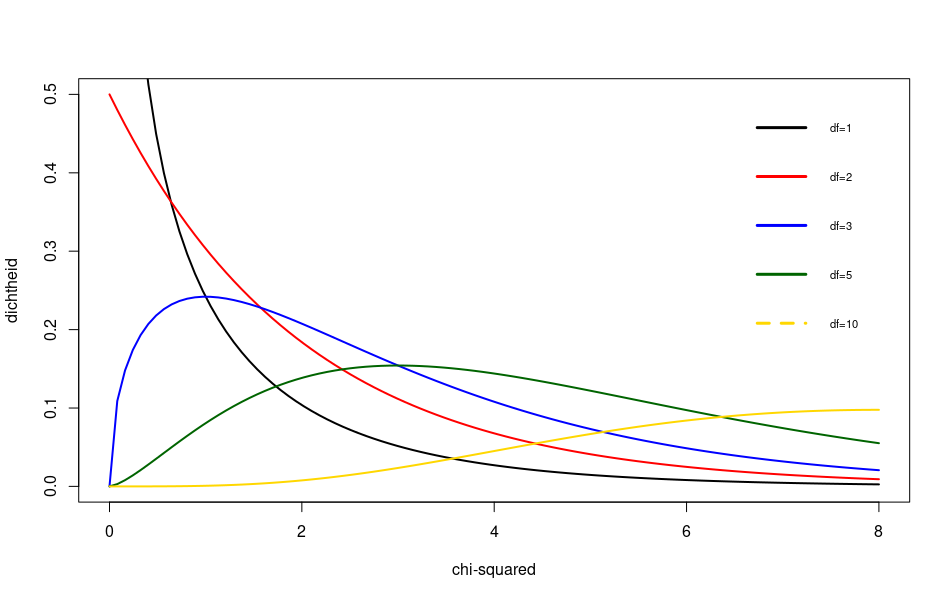
\includegraphics[width=\textwidth]{chi-squared-distribution}
  \caption{Dichtheidsfunctie van de $\chi^2$-verdeling voor verschillende vrijheidsgraden $df$.}
  \label{fig:chi-squared-distribution}
\end{figure}

\subsection{Onafhankelijkheidstoets}
\label{ssec:onafhankelijkheidstoets}

Een onafhankelijkheidstoets\index{onafhankelijkheidstoets} gaat na of er een verband bestaat tussen twee kwalitatieve variabelen aan de hand van de $\chi^2$-statistiek. Deze toets wordt ook de $\chi^2$-toets\index{$\chi^2$-toets!}\index{toets!$\chi^2$-} voor associatie genoemd, of de $\chi^2$-kruistabeltoets, en is ontwikkeld door de Engelse wiskundige en statisticus Karl Pearson\index{Pearson!Karl}.

\subsubsection{Toetsingsprocedure}

De toetsingsprocedure verloopt als volgt:

\begin{enumerate}
  \item \textbf{Bepalen hypotheses}
  Als nulhypothese stellen we dat er geen verband is tussen de onafhankelijke en de afhankelijke variabele (en verwachten we dus een kleine $\chi^2$). Als alternatieve hypothese stellen we dat er \emph{wel} een verband is (en dat $\chi^2$ dus groot is).
  \begin{itemize}
    \item $H_{0}$: er is geen verband tussen de variabelen (of: de variabelen zijn onafhankelijk)
    \item $H_{1}$: er is een verband tussen de variabelen
  \end{itemize}

  \item \textbf{Bepalen significantieniveau $\alpha$}
  
  \item \textbf{Bereken de waarde van de toetsingsgrootheid in de steekproef}
  \[ \chi^{2} = \sum_{i} \frac{(o_{i} - e_{i})^{2}}{e_{i}} \]
  
  \item De waarde van $\chi^2$ is gedistribueerd volgens de $\chi^2$-verdeling (zie Sectie~\ref{ssec:chi-kwadraatverdeling}). Deze stochastische verdeling heeft als bijkomende parameter het aantal vrijheidsgraden $df$. Voor een kruistabeltoets is $df = (r - 1) \times (k - 1)$ met $r$ het aantal rijen en $k$ het aantal kolommen.
  
  Aan de hand van deze verdeling kunnen we op twee equivalente manieren een besluit trekken:
  
  \begin{enumerate}
    \item \textbf{Bereken en teken kritiek gebied}. De kritieke grenswaarde $g$ is het getal waarvoor geldt dat $P(\chi^2 > g) = \alpha$. Deze toets is altijd rechtszijdig. Als $\chi^2 < g$, dan zitten we in het \emph{aanvaardingsgebied}, waar we de nulhypothese niet kunnen verwerpen. Als $\chi^2 > g$, dan zitten we in het \emph{verwerpingsgebied} en zullen we de nulhypothese verwerpen.
    \item \textbf{Bereken de overschrijdingskans $p$}. Dit is de rechterstaartkans voor de bekomen $\chi^2$-statistiek in de steekproef, afhankelijk van het aantal vrijheidsgraden. De interpretatie van de $p$-waarde is ``Als we zouden veronderstellen dat er \emph{geen} verband is tussen de twee variabelen, wat is dan de kans dat ik een waarde voor $\chi^2$ tegenkom in een steekproef die minstens zo groot is als de daarnet berekende?'' Als $p > \alpha$ (en dus de kans relatief groot is dat we deze $ \chi^2$-waarde tegenkomen), dan aanvaarden we de nulhypothese, als $p < \alpha$, dan verwerpen we deze.
  \end{enumerate}

  \item Tenslotte formuleren we de conclusie en beantwoorden we de onderzoeksvraag.
\end{enumerate}

Toegepast op het voorbeeld van hierboven:

\begin{enumerate}
  \item \textbf{Bepalen hypotheses:}
  \begin{itemize}
    \item $H_0$ Er is geen verband tussen gender en waardering
    \item $H_1$ Er is een verband tussen gender en waardering
  \end{itemize}
  \item \textbf{Bepalen significantieniveau:} $\alpha = 0,05$
  
  \item \textbf{Bereken de waarde van de toetsingsgrootheid in de steekproef}
  
  $\chi^2 \approx 3,8105$ (zie Sectie~\ref{ssec:chi-kwadraat})
  
  \item Bepaal het aantal vrijheidsgraden $df = (r - 1) \times (k - 1) = (4 - 1) \times (2 - 1) = 3$.
  
  \begin{enumerate}
    \item \textbf{Bepaal de kritieke grenswaarde:} $g \approx 7,815$. In dit geval is $\chi^2 < g$, dus we zitten in het aanvaardingsgebied. We kunnen $H_0$ dus niet verwerpen.
    \item \textbf{Bereken de overschrijdingskans:} $p \approx 0,2827$. Er is dus een kans van ongeveer 28\% dat we deze $\chi^2$-waarde tegenkomen. Dat is vrij groot, zeker al groter dan $\alpha$. Bijgevolg kunnen we $H_0$ niet verwerpen.
  \end{enumerate}

  \item We kunnen dus besluiten dat er op basis van deze steekproef geen reden is om aan te nemen dat er een verband is tussen gender en waardering. Anders gezegd, er zijn geen significante verschillen tussen de waarderingen bij enerzijds vrouwen en anderzijds mannen.
\end{enumerate}


We geven nog een ander voorbeeld van de onafhankelijkheidstoets aan de hand van een studie door \textcite{Doll1954} over de relatie tussen roken en longkanker. Doll en Hill schreven in 1951 alle Britse huisartsen aan met het verzoek om gegevens over hun leeftijd en rookgedrag. Vervolgens hielden ze jarenlang de overlijdensberichten en de doodsoorzaak bij en herhaalden hun periodiek. De eerste uitkomsten, na circa vier jaar, zijn in tabel~\ref{tab:dollhill} samengevat. Uit de tabel kan makkelijk geconcludeerd worden dat er geen relatie is tussen roken en longkanker. In (ruim) vier jaar is slechts $(84 / 24354) * 100 = 0,35\%$ van de Britse artsen aan longkanker overleden en dat met slechts $(83 / 21261) * 100 = 0,39\%$ van de rokers onder hen. Dit is weinig, maar het is wel veel meer dan hetzelfde cijfer voor de niet-rokers $(1 / 3093) * 100 = 0,032\%$.

\begin{table}
  \begin{center}
    \begin{tabular}{@{}lllll@{}}
    	\toprule
    	               & \textbf{Longkanker} & \textbf{Niet} & \textbf{Wel} & \textbf{Totaal} \\
    	\midrule
    	\textbf{Roker} & \textbf{Wel}        & 21178         & 83           & 21261           \\
    	               & \textbf{Niet}       & 3092          & 1            & 3093            \\
    	               & \textbf{Totaal}     & 24270         & 84           & 24354           \\
    	\bottomrule
    \end{tabular}
  \end{center}
  \caption{Resultaten van het onderzoek van~\textcite{Doll1954}}
  \label{tab:dollhill}
\end{table}

We zien in de tabel dat er wel een erg groot verschil is tussen de geobserveerde aantallen rokers die overlijden aan longkanker en de verwachte frequenties in deze cel. Hetzelfde geldt voor het geringe aantal huisartsen dat niet rookt, maar wel aan longkanker overleden is. Deze observatie maakt ons wel wantrouwig of de eerdere tentatieve conclusie wel juist is. We kunnen afrekenen met deze onzekerheid door de toetsingsgrootheid $\chi^{2}$ uit te rekenen. Dat doen we op de vertrouwde manier:

\begin{enumerate}
  \item \textbf{Bepalen hypotheses}
  \begin{itemize}
    \item $H_{0}$: er is geen verband tussen roken en sterven aan longkanker
    \item $H_{1}$: er is een verband tussen roken en sterven aan longkanker
  \end{itemize}
  \item \textbf{Bepalen $\alpha$ en $n$:} $\alpha = 0,05$ en $n = 24354$.
  \item \textbf{Toetsingsgrootheid en waarde ervan in steekproef}:
  \[ \chi^{2} = \sum_{i=1}^{k \times r} \frac{(o_{i} - e_{i})^{2}}{e_{i}} \approx 10,071 \]
  \item \textbf{Bereken en teken kritiek gebied}: Het aantal vrijheidsgraden is $df = (r-1)(k-1) = 1$, dus voor het gegeven significantieniveau is de kritieke grens 3,8415. Onze toetsingsgrootheid ligt in het kritieke gebied dus verwerpen we $H_{0}$.
\end{enumerate}

We moeten derhalve $H_{0}$, dat er geen relatie is tussen beide variabelen, verwerpen ten gunste van $H_{1}$ dat er wel een relatie is tussen beide variabelen: rokers sterven vaker aan longkanker dan niet-rokers.

Maar, is dit nu een bewijs dat zoals zo vaak verondersteld wordt dat roken longkanker \emph{veroorzaakt}? Nee, dat is het absoluut niet. Een paar alternatieve verklaringen: niet alle rokers krijgen longkanker, de rokers zijn ouder dan de niet-rokers, de rokers wonen veelal in de grote steden met meer vervuilde lucht dan de niet-rokers die veelal op het platte land wonen, ook zou er nog een speciale genetische dispositie kunnen zijn, die zowel van invloed is op de verslaving aan tabak, als op de kans om longkanker te krijgen. Voor een causale interpretatie van de gegevens (let wel, het betreft hier immers geen experiment), moeten we op zijn minst de beschikking hebben over een theorie die de relatie tussen roken en longkanker expliciteert.

\begin{remark}[!!]
  \textbf{Correlation is not causation.} Of anders gezegd, een verband tussen twee variabelen impliceert niet dat er ook een \emph{oorzakelijk} verband is. Dit is een erg vaak voorkomende fout die gemaakt wordt wanneer journalisten een artikel schrijven over resultaten van wetenschappelijk onderzoek. Wees hier dus alert voor wanneer je dergelijke artikels leest!
\end{remark}

\subsubsection{De regel van Cochran}

Bij het berekenen van de $\chi^2$-waarde is het belangrijk dat er voor elke cel in de kruistabel voldoende observaties beschikbaar zijn. Als de steekproef te klein is, zullen de resultaten van de berekening onbetrouwbaar worden.

De statisticus \textcite{Cochran1954}\index{Cochran!William G.} heeft hierover een aantal aanbevelingen geformuleerd die we in deze cursus de Regel van Cochran\index{Cochran!regel van} zullen noemen.

Om de $\chi^2$-toets te mogen toepassen moeten specifiek de volgende voorwaarden vervuld zijn:

\begin{enumerate}
  \item Voor alle categorie\"en moet gelden dat de verwachte frequentie $e$ groter is dan 1.
  \item In ten hoogste 20 \% van de categorie\"en mag de verwachte frequentie $e$ kleiner dan 5 zijn.
\end{enumerate}

\subsection{Aanpassingstoets}
\label{ssec:aanpassingstoets}

De $\chi^2$-toets kan ook worden toegepast wanneer je wil nagaan of een bepaalde discrete verdeling (bv. de frequenties van een enkele kwalitatieve variabele) al dan niet overeenkomen met een gekende verdeling. Deze variant noemen we de \emph{aanpassingstoets}\index{aanpassingstoets} of in het Engels de \emph{goodness-of-fit test}\index{goodness-of-fit test}. Deze toets wordt vaak toegepast om na te gaan of de verdeling van een bepaalde kwalitatieve variabele in een steekproef representatief is voor de populatie, in de veronderstelling dat je weet welke frequenties er in de populatie als geheel voorkomen.

Stel, in het onderzoek naar onze superhelden is een steekproef genomen van $n = 400$ observaties. De onderzoekers willen weten of de voorkomende types van superhelden in de steekproef overeenkomen met die in de populatie, m.a.w.~of de steekproef representatief is. Tabel~\ref{tab:frequenties-types-superhelden} geeft een overzicht van de geobserveerde frequenties in de steekproef en de verwachte frequenties in de populatie.

\begin{table}
  \centering
  \begin{tabular}{@{}lcc@{}}
  	\toprule
  	\textbf{Type}   & \textbf{frq steekproef ($o$)} & \textbf{frq populatie ($\pi$)} \\
  	\midrule
  	Mutant          &              127              &              35\%              \\
  	Mens            &              75               &              17\%              \\
  	Alien           &              98               &              23\%              \\
  	God             &              27               &              8\%               \\
  	Demon           &              73               &              17\%              \\
  	\midrule
  	\textbf{Totaal} &              400              &             100\%
  \end{tabular}
  \caption{Absolute frequenties van de types superhelden in de steekproef ($o$) en verwachte relatieve frequenties ($\pi$) in de populatie als geheel.}
  \label{tab:frequenties-types-superhelden}
\end{table}

We willen de frequenties in de steekproef vergelijken met de aantallen die je zou verwachten als de steekproef exact representatief zou zijn naar de types van superhelden. Als deze verschillen relatief groot zijn dan komt de verdeling in de steekproef \emph{niet} overeen met de verdeling in de populaties en zullen we moeten concluderen dat de steekproef niet representatief is. Om te oordelen of deze verschillen relatief groot zijn, voeren we een $\chi^{2}$-toets uit.

Als de steekproef exact representatief is, dan zouden we verwachten dat in de steekproef 35\% van de superhelden een mutant is. Het verwachte aantal of de verwachte frequentie voor deze categorie is dus gelijk aan $0,35 \times 400 = 140$. Er geldt dus:

\[ e = n \times \pi \]

met $e$ de verwachte absolute frequentie in de steekproef, $n$ de steekproefgrootte en $\pi$ de verwachte relatieve frequentie voor de hele populatie. Als de verschillen tussen de geobserveerde en verwachte frequenties $(o - e)$ relatief klein zijn, kunnen ze toegerekend worden aan toevallige steekproeffouten. We kunnen opnieuw $\chi^2$ gebruiken om deze verschillen samen te vatten en te interpreteren:

\[ \chi^{2} = \sum_i \frac{(o_{i} - e_{i})^{2}}{e_{i}} \]

We merken op:

\begin{itemize}
  \item indien de verschillen klein zijn $\Rightarrow$ verdeling is representatief
  \item indien de verschillen groot $\Rightarrow$ verdeling niet representatief
\end{itemize}

We bepalen nu een kritieke grenswaarde $g$ die een $\chi^{2}$ verdeling heeft. Hierbij speelt het aantal vrijheidsgraden ($df$) een rol. Voor deze toets geldt:

\[ df = k - 1 \]

met $k$ het aantal categorie\"en. In ons voorbeeld hebben we $df = 5-1 = 4$. Om de kritieke grenswaarde te bepalen, kan je gebruik maken van een tabel voor de $\chi^2$-verdeling. Voor een gegeven significantieniveau $\alpha$ en vrijheidsgraad $df$ kan je in zo'n tabel de grenswaarde aflezen.

In ons voorbeeld is $\chi^{2} = 3,47$ met grenswaarde $g = 9,49$. Omdat de gevonden toetsingsgrootheid $\chi^2 = 3,47 < g = 9,49$, mogen we besluiten dat de steekproef representatief is.

\subsubsection{Toetsingsprocedure}

We volgen de stappen van een statistische toetsingsprocedure:

\begin{enumerate}
  \item \textbf{Bepalen hypotheses}
  Als nulhypothese formuleren we dat de steekproef representatief is, meer bepaald dat de verdeling in de steekproef gelijk is aan de verdeling over de populatie. Als alternatieve hypothese formuleren we dat de verdelingen verschillend zijn.
  \begin{itemize}
    \item $H_{0}$: steekproef is representatief voor de populatie
    \item $H_{1}$: steekproef is niet representatief voor de populatie
  \end{itemize}
  \item \textbf{Bepalen $\alpha$ en $n$}
  \item \textbf{Waarde van de toetsingsgrootheid in de steekproef}:
  \[ \chi^{2} = \sum_{i=1}^{n} \frac{(o_{i} - e_{i})^{2}}{e_{i}} \]
  \item Bepaal het aantal vrijheidsgraden $df = k - 1$ met $k$ het aantal categorieën
  \begin{enumerate}
    \item \textbf{Bereken en teken kritiek gebied}: de toets is altijd rechtszijdig. Is de toetsingsgrootheid kleiner dan kritieke grenswaarde $\chi^2 < g$, verwerp $H_{0}$ niet. Als $\chi^2 > g$, verwerp $H_{0}$ en aanvaard $H_{1}$.
    \item \textbf{Bereken de overschrijdingskans $p$}. Als $p > \alpha$, dan aanvaarden we de nulhypothese, als $p < \alpha$, dan verwerpen we deze.
  \end{enumerate}
  \item Formuleer tenslotte het antwoord op de onderzoeksvraag.
\end{enumerate}

\subsubsection{Gestandaardiseerde residuen}

We bespreken nog een ander voorbeeld. Beschouw alle gezinnen met precies 5 kinderen in een bepaalde gemeenschap. Wat betreft het aantal jongens/meisjes in zo'n gezin zijn er 6 mogelijkheden:

\begin{enumerate}
  \item 5 jongens
  \item 4 jongens, 1 meisje
  \item 3 jongens, 2 meisjes
  \item 2 jongens, 3 meisjes
  \item 1 jongen, 4 meisjes
  \item 5 meisjes
\end{enumerate}

Stel dat er een onderzoek gebeurd is waar 1022 gezinnen met 5 kinderen hebben aan deelgenomen. In Tabel~\ref{tab:5-kinderen} worden de frequenties gegeven van het aantal jongens in elk gezin. Zijn de waargenomen aantallen in de 6 klassen representatief voor een populatie waar de kans om een jongen te krijgen gelijk is aan de kans om een meisje te krijgen, nl.~0,5?

\begin{table}
  \centering
  \begin{tabular}{@{}cccccccc@{}}
    \toprule
    i       & 0  & 1   & 2   & 3   & 4   & 5  &  \\
    \midrule
    $o_{i}$ & 58 & 149 & 305 & 303 & 162 & 45 &  \\
    \bottomrule
  \end{tabular}
  \caption{Frequenties $o_i$ van het aantal jongens $i$ in gezinnen met vijf kinderen uit een onderzoek met $n = 1022$ gezinnen.}
  \label{tab:5-kinderen}
\end{table}

Indien de veronderstelling waar is, wordt de kans $\pi_{i}$ om $i$ jongens te krijgen bepaald door een binominaalverdeling met parameters $n=5$ en $p=0,5$.

Dit kan je eenvoudig nagaan aan de hand van het voorbeeld. De kans om 2 jongens te krijgen met 5 kinderen is gelijk aan :

\[ (0,5)^{2} \times (1-0,5)^{5-2} \times \binom{5}{2} \]

Algemeen geldt dus:

\[ \pi_{i} = \binom{5}{i}\times 0,5^{i} \times 0,5^{5-i} = \frac{5!}{i!(5-i)!}\times 0,5^{5} \]

Met deze $\pi_{i}$ kunnen we dus de verwachte frequentie $e$ bepalen en de stappen volgen zoals hierboven beschreven. Tabel~\ref{tab:5-kinderen-berekeningen} geeft een overzicht van de nodige berekeningen.

\begin{table}
  \centering
  \begin{tabular}{@{}lrrrrrrr@{}}
  	\toprule
  	$i$                   &     0 &      1 &      2 &      3 &      4 &     5 &  Tot. \\
  	\midrule
  	$o_i$                 &    58 &    149 &    305 &    303 &    162 &    45 &  1022 \\
  	$\pi_i$               &  0,03 &   0,15 &   0,31 &   0,31 &   0,15 & 0,031 &     1 \\
  	$e_i$                 & 31,68 & 159,43 & 318,86 & 318,86 & 159,43 & 31,68 &       \\
  	$\frac{(o-e)^{2}}{e}$ & 21,86 &   0,68 &   0,60 &   0,78 &   0,04 &  5,59 & 29,57 \\
  	$r_i$                 &  4,74 &  -0,89 &  -0,93 & -1,071 &   0,22 &  2,40 &       \\
  	\bottomrule
  \end{tabular}
  \caption{Berekeningen voor de casus van gezinnen met 5 kinderen. $i$ is het aantal jongens in het gezin, $o_i$ de geobserveerde aantallen gezinnen in de steekproef met $i$ jongens. $\pi_i$ is de verwachte kans dat in een gezin van 5 kinderen $i$ jongens voorkomen en $e_i$ de verwachte frequentie. Daaronder wordt nog de berekening van $\chi^2$ getoond en tenslotte de gestandaardiseerde residuën $r_i$.}
  \label{tab:5-kinderen-berekeningen}
\end{table}

\begin{enumerate}
  \item \textbf{Bepalen hypotheses}
  
  \begin{itemize}
    \item $H_{0}$: de steekproef is representatief voor de populatie
    \item $H_{1}$: de steekproef is niet representatief voor de populatie
  \end{itemize}
  \item \textbf{Bepalen $\alpha$ en $n$} : $\alpha = 0,01$ en $n = 1022$.
  \item \textbf{Toetsingsgrootheid en waarde ervan in steekproef}:
  \[ \chi^{2} = \sum_{i=1}^{n} \frac{(o_{i} - e_{i})^{2}}{e_{i}} = 29,5766 \]
  \item \textbf{Bereken en teken kritiek gebied}:  kritieke grens is 15,0863. Onze toetsingsgrootheid ligt dus in het kritieke gebied dus verwerpen we $H_{0}$. 
\end{enumerate}

We vinden dus dat de steekproef \emph{niet} representatief is voor een populatie waar geldt dat de kans op een jongen even groot is als de kans op een meisje.

Nu kunnen we ons de vraag stellen of \emph{elke} klasse afwijkt van de verwachte frequentie, of slechts één of enkele. Welke klassen zijn er onder- of oververtegenwoordigd in de steekproef? Om dit te bepalen, gebruiken we de zgn.~\emph{gestandaardiseerde residuen}\index{residuen!gestandaardiseerde} die aanduiden welke klassen de grootste bijdrage leveren aan de waarde van $\chi^2$. 

\[ r_{i} = \frac{O_{i} - n \pi_{i}}{\sqrt{n \pi_{i}(1-\pi_{i})}} \]

%\begin{exercise}
%  Hoe komen we hier aan de noemer? Waar komt dit mee overeen? Hoe bepaal je de variantie van een binomiale verdeling?
%  
%  Antwoord: $n \times \pi (1-\pi)$
%\end{exercise}

De waarde voor $r_i$ is 0 als $o = e$. Negatieve waarden wijzen er op dat deze klasse ondervertegenwoordigd is in de steekproef, positieve dat ze oververtegenwoordigd is. Er geldt algemeen dat waarden groter dan 2 of kleiner dan $-2$ extreem zijn. We kunnen dus uit Tabel~\ref{tab:5-kinderen-berekeningen} besluiten dat het aantal gezinnen met enkel jongens ($r_5 = 2,4$) of enkel meisjes ($r_0 = 4,74$) groter mag worden genoemd dan verwacht.

\subsection{Cramér's V}
\label{ssec:cramers-v}

Uit de grootte van de $\chi^2$-statistiek is het niet meteen mogelijk om af te leiden of er een verband tussen beide variabelen bestaat. Dit hangt af van de grootte van de kruistabel, meer bepaald het aantal rijen en kolommen.

De Zweedse wiskundige en statisticus Harald Cramér\index{Cramér!Harald} heeft een metriek ontwikkeld die de $\chi^2$ voor gelijk welke kruistabel herleidt tot een waarde tussen 0 en 1, Cramér's V\index{Cramér's V}:

\begin{definition}[Cramér's V]
  \begin{equation}
  V = \sqrt{\frac{\chi^{2}}{n (k-1)}}
  \label{eq:Cramer}
  \end{equation}
  met
  \begin{itemize}
    \item $\chi^{2}$ de berekende chi-kwadraatwaarde.
    \item $n$ het aantal waarnemingen (steekproefgrootte).
    \item $k$ = de kleinste waarde van het aantal kolommen of het aantal rijen van de tabel.
  \end{itemize}
  
\end{definition}

Cramér's V is de $\chi^{2}$, gecorrigeerd voor steekproefomvang en het aantal categorieën in de variabelen. Tabel~\ref{tab:interpretatie-cramers-v} geeft aan hoe je het resultaat kan interpreteren.

\begin{table}
  \centering
  \begin{tabular}{ll}
    $V = 0$ & geen samenhang \\
    $V \approx 0,1$ & zwakke samenhang \\
    $V \approx 0,25$ & redelijk sterke samenhang \\
    $V \approx 0,50$ & sterke samenhang \\
    $V \approx 0,75$ & zeer sterke samenhang \\
    $V = 1$ & volledige samenhang \\
  \end{tabular}
  \caption{Interpretatie van de waarde van Cramérs'V}
  \label{tab:interpretatie-cramers-v}
\end{table}

Voor onze eerdere casus waar werd onderzocht of er een verband was tussen gender en waardering vonden we een $\chi^{2} \approx 3,811$. Cramér's V is dan $\sqrt{\frac{3,811}{49 (2 - 1)}} \approx 0,279$. Dit duidt op redelijk sterke samenhang tussen de variabelen. Met andere woorden, de resultaten van de bevraging geven aan dat er een verschil is in de waardering die vrouwen en mannen geven over het assortiment.

Dit resultaat is opmerkelijk omdat we via de $\chi^2$-toets geen significant verband gevonden hebben tussen beide variabelen. Het is bekend dat Cramér's V de neiging heeft om de mate van associatie te overschatten. Het is dus mogelijk dat dat ook in dit geval gebeurd is.

\begin{example}
  In Tabel~\ref{tab:autovoorkeur} worden de voorkeuren van vrouwen en mannen voor de gegeven automerken opgesomd. We zien dat nog steeds dertig van de honderd respondenten een voorkeur hebben voor de Mercedes, maar dat twee derde van deze dertig vrouwen zijn. We zouden  ook kunnen zeggen dat de helft van de vrouwen een voorkeur heeft voor de Mercedes. Evenzo blijkt dat een derde van de mannen een voorkeur heeft voor een Alfa Romeo, tegenover geen van de vrouwen. Het lijkt alsof de onderscheiden automerken niet gelijkelijk gewaardeerd worden door mannen en vrouwen. Om dit te staven bepalen we $\chi^{2}$ en Cramér's V. Probeer dit zelf, hetzij in R, hetzij met een rekenblad (Excel, Numbers, LibreOffice Calc)! We vinden:
  \[ \chi^{2} = 22,619 \]
  \[ V = \sqrt{\frac{22,619}{100 \times (2-1)}}  = 0,476\]
  
  We vinden dus tussen een redelijk sterke tot sterke samenhang.
\end{example}

\begin{table} \centering
  \begin{tabular}{@{}rrrrrr@{}}
  	\toprule
  	        & Mercedes &  BMW & Porsche & Alfa Romeo & Totaal \\
  	\midrule
  	 Mannen &     $10$ & $10$ &    $20$ &       $20$ &   $60$ \\
  	Vrouwen &     $20$ &  $5$ &    $15$ &        $0$ &   $40$ \\
  	 Totaal &     $30$ & $15$ &    $35$ &       $20$ &  $100$ \\
  	\bottomrule
  \end{tabular}
  \caption{Tabel die uitdrukt hoeveel vrouwen en hoeveel mannen een voorkeur voor een bepaald automerk hebben.}
  \label{tab:autovoorkeur}
\end{table}

\subsection{Visualisatietechnieken}
\label{ssec:kwal-kwal-visualisatie}

\subsection{Geclusterd staafdiagram}
\subsection{Rependiagram}
\subsection{Mozaïekdiagram}

\section{Kwalitatief--kwantitatief}
\label{sec:kwal-kwant}

In deze sectie bekijken we methoden om na te gaan of er een verband bestaat tussen enerzijds een kwalitatieve variabele (onafhankelijk) en anderzijds een kwantitatieve variabele (afhankelijk). Een onderzoek naar genderongelijkheid bij verloning in de ict-sector is hier een goed voorbeeld van. De onafhankelijke variabele \emph{gender} is nominaal (mogelijke waarden bijvoorbeeld M/V/X), de afhankelijke variabele \emph{netto maandloon} is een ratio-variabele.

De benadering die men typisch gebruikt, is om het gemiddelde en/of standaardafwijking van de afhankelijke variabele tussen de verschillende groepen ontstaan uit de onafhankelijke met elkaar te vergelijken. Als de verschillen klein zijn, dan kunnen ze worden toegeschreven aan toevallige steekproeffouten en besluiten we dat er geen verband is. Als de verschillen groot zijn, dan besluiten we dat er \emph{wel} een verband is. Vaak is het bijvoorbeeld nog altijd zo dat mannen significant meer verdienen dan vrouwen voor een gelijkaardige job!

In deze cursus bespreken we de $t$-toets voor 2 steekproeven om te bepalen of er een verschil is tussen twee groepen (zie Sectie~\ref{ssec:t-toets-twee-steekproeven}). Er bestaan statistische toetsen om een groter aantal groepen tegelijk te beschouwen (bijvoorbeeld de ANOVA-toets), maar die vallen buiten het bestek van deze cursus.

Net zoals Cramér's V bij kwalitatieve variabelen bestaan er ook in dit geval metrieken die aangeven hoe sterk het verband is tussen kwalitatieve en kwantitatieve variabelen. In deze context worden die vaak onder de noemer \emph{effectgrootte} genoemd. In deze cursus zien we één definitie van effectgrootte, nl.~Cohen's $d$ (zie Sectie~\ref{ssec:cohens-d}). Opnieuw, er bestaan meerdere vormen van effectgrootte, ook geschikt voor variabelen met andere meetniveaus, maar deze vallen ook buiten het bestek van deze cursus.

\subsection{De \texorpdfstring{$t$}{t}-toets voor twee steekproeven}
\label{ssec:t-toets-twee-steekproeven}

De $t$-toets die geïntroduceerd werd in Sectie~\ref{sec:t-toets} kan ook gebruikt worden om twee steekproeven met elkaar te vergelijken. Je kan er dan mee nagaan of het steekproefgemiddelde van beide steekproeven \emph{significant} verschillend is.

Men maakt onderscheid tussen twee gevallen:

\begin{itemize}
  \item Beide steekproeven zijn onafhankelijk, zijn afzonderlijk genomen. Een voorbeeld is een onderzoek naar een medische behandelingsmethode waar een contolegroep de behandeling \emph{niet} krijgt en een testgroep de behandeling wel krijgt.
  \item De steekproeven zijn afhankelijk, of gepaard. Een voorbeeld is twee metingen uitvoeren op hetzelfde lid van de populatie, zoals de koorts nemen voor en na het innemen van een medicijn om het effect ervan te meten.
\end{itemize}

In R kan je eveneens de functie \texttt{t.test} gebruiken voor het uitvoeren van een toets met twee steekproeven. We geven hieronder twee voorbeelden, één voor elk geval.

\begin{example}
  In een klinisch onderzoek wil men nagaan of een nieuw medicijn als bijwerking een vertraagde (dus hogere) reactiesnelheid heeft~\autocite{Lindquist}.
  
  Zes deelnemers kregen een medicijn toegekend (interventiegroep) en zes anderen een placebo (controlegroep). Vervolgens werd hun reactietijd op een stimulus gemeten (in ms). We willen nagaan of er significante verschillen zijn tussen de interventie- en controlegroep.
  
  \textbf{Opmerking}: De interventiegroep en de controle groep zijn hier toevallig even groot (elk 6 proefpersonen).
  Dit is niet noodzakelijk. Bij een onafhankelijke (niet-gepaarde) steekproeven
  mogen de 2 groepen een verschillende grootte hebben.
  
  \begin{itemize}
    \item Controlegroep: 91, 87, 99, 77, 88, 91 ~~~~~~~~~~~~($\overline{x}=88,83$)
    \item Interventiegroep: 101, 110, 103, 93, 99, 104 ~~($\overline{y}=101,67$)
  \end{itemize}
  
  We noteren $\mu_1$ voor het gemiddelde van de niet behandelde populatie (controlegroep) en $\mu_2$ voor het populatiegemiddelde van de patiënten die het medicijn nemen (interventiegroep).
  
  De hypothesen worden formeel als volgt genoteerd:
  
  $H_0: \mu_1 - \mu_2 = 0$ en $H_1: \mu_1 - \mu_2 < 0$
  
  Als toetsingsgrootheid gebruiken we $\overline{x}-\overline{y}$, met $\overline{x}$ en $\overline{y}$ schattingen voor de \textit{\'echte} waarden $\mu_1$ en $\mu_2$ .
  
  Het gaat hier dus over een linkszijdige test, wat weergegeven wordt door de optie \texttt{alternative = "less"}. In de nulhypothese veronderstellen we dat het verschil tussen de populatiegemiddelden 0 is, wat met de optie \texttt{mu = 0} wordt aangeduid. Merk op dat dit de standaardwaarde is voor deze parameter en dus in principe niet moet worden opgegeven.
  
  \begin{lstlisting}
  controle <-  c(91, 87, 99, 77, 88, 91)
  interventie <- c(101, 110, 103, 93, 99, 104)
  t.test(controle, interventie, alternative="less", mu=0)
  \end{lstlisting}
  
  Het resultaat van de toets:
  
  \begin{verbatim}
  t.test(controle, interventie, alternative="less")
  
  Welch Two Sample t-test
  
  data:  controle and interventie
  t = -3.4456, df = 9.4797, p-value = 0.003391
  alternative hypothesis: true difference in means is less than 0
  95 percent confidence interval:
  -Inf -6.044949
  sample estimates:
  mean of x mean of y 
  88.83333 101.66667
  \end{verbatim}
  
  De teststatistiek $\overline{x}-\overline{y}=-12,833$ komt overeen met een $t$-waarde $t=-3,4456$.
  De parameter $df=9,48$ wordt bepaald door \texttt{t.test()} op basis van
  het aantal elementen in de reeksen $x$ en $y$.
  De berekening hiervan is \textit{niet} triviaal.
  
  De $p$-waarde, 0,003391, ligt duidelijk onder het significantieniveau (niet expliciet opgegeven, dus werd de standaardwaarde $\alpha = 0,05$ gebruikt.)
  
  We mogen dus de nulhypothese verwerpen en besluiten dat volgens de resultaten van deze steekproef het medicijn inderdaad een significant effect heeft op de reactiesnelheid van patiënten.
  
  \textbf{Opmerking}: Vermits $\overline{x}-\overline{y}=-12,833$
  kunnen we met 95\% procent zekerheid zeggen dat het verschil van de \textit{\'echte} gemiddelden ($\mu_1-\mu_2$)
  van een grotere controle- en interventiepopulatie tussen $-\infty$ en $-6.044949$ zal liggen.
  Zie paragraaf \ref{ssec:betrouwbaarheidsinterval-grote-steekproef} (p. \pageref{ssec:betrouwbaarheidsinterval-grote-steekproef})
  en \ref{ssec:betrouwbaarheidsinterval-kleine-steekproef} (p. \pageref{ssec:betrouwbaarheidsinterval-kleine-steekproef})
  over betrouwbaarheidsintervallen.
\end{example}

\begin{example}
  In een studie werd nagegaan of auto's die rijden op benzine met additieven ook een lager verbruik hebben. Tien auto's werden eerst volgetankt met ofwel gewone benzine, ofwel benzine met additieven (bepaald door opgooien van een munt), waarna het verbruik werd gemeten (uitgedrukt in mijl per gallon). Vervolgens werden de auto's opnieuw volgetankt met de andere soort benzine en werd opnieuw het verbruik gemeten. De resultaten worden gegeven in de tabel hieronder.
  
  \begin{center}
    \begin{tabular}{|l|c|c|c|c|c|c|c|c|c|c|}
      \hline 
      Auto & 1 & 2 & 3 & 4 & 5 & 6 & 7 & 8 & 9 & 10 \\ 
      \hline 
      Gewone benzine & 16 & 20 & 21 & 22 & 23 & 22 & 27 & 25 & 27 & 28 \\ 
      \hline 
      Additieven & 19 & 22 & 24 & 24 & 25 & 25 & 25 & 26 & 28 & 32 \\ 
      \hline 
    \end{tabular} 
    %  \caption{Verbruik in mijl per gallon met 2 soorten benzine.}
    %  \label{tab:benzineverbruik-additieven}
  \end{center}
  
  We gaan door middel van een \emph{gepaarde $t$-test} na of auto's significant zuiniger rijden met benzine met additieven.
  
  We kiezen $x$ voor benzine met \texttt{additieven} ($\overline{x}=25,1$ mijl per gallon), en we kiezen $y$ voor \texttt{gewone} bezine ($\overline{y}=23,1$ mijl per gallon).
  
  De nulhypothese $H_0$ is dat je met beiden even veel mijl per gallon kunt rijden ($\mu_{x-y}=0$).
  De alternatieve hypothese $H_1$ dat je verder kunt rijden op benzine met additieven ($\mu_{x-y}>0$).
  
  De optie \texttt{paired=TRUE} geeft aan dat het hier om een gepaarde $t$-toets gaat.
  
  \begin{lstlisting}
  gewone    <- c(16, 20, 21, 22, 23, 22, 27, 25, 27, 28)
  additieven <-c(19, 22, 24, 24, 25, 25, 26, 26, 28, 32)
  t.test(additieven, gewone, alternative="greater", paired=TRUE)
  \end{lstlisting}
  
  Resultaat:
  
  \begin{verbatim}
  Paired t-test
  
  data:  additieven and gewone
  t = 4.4721, df = 9, p-value = 0.0007749
  alternative hypothesis: true difference in means is greater than 0
  95 percent confidence interval:
  1.180207      Inf
  sample estimates:
  mean of the differences 
  2 
  \end{verbatim}
  
  De teststatistiek $\overline{x-y}=2$. Dit komt overeen met een $t$-waarde $t=4,4721$.
  De $p$-waarde, 0,0007749, ligt onder het significantieniveau ($\alpha=0,05$), dus we kunnen de nulhypothese verwerpen. Volgens deze steekproef rijden auto's inderdaad zuiniger met benzine met additieven.
  
  \textbf{Ter info}: Bij 95\% van de ``paren'' van een grotere populatie auto's,
  zal het verschil $x-y$ tussen $1.180207$ en $+\infty$ liggen.
  Dit is het betrouwbaarheidsinterval waarvan sprake in paragraaf \ref{ssec:betrouwbaarheidsinterval-grote-steekproef} (p. \pageref{ssec:betrouwbaarheidsinterval-grote-steekproef})
  en \ref{ssec:betrouwbaarheidsinterval-kleine-steekproef} (p. \pageref{ssec:betrouwbaarheidsinterval-kleine-steekproef}).
\end{example}

\subsection{Effectgrootte - Cohen's \texorpdfstring{$d$}{d}}
\label{ssec:cohens-d}

Met de term \emph{effectgrootte}\index{effectgrootte} bedoelt men een metriek die de impact (of effect) van een gebeurtenis weergeeft. Bij de meeste varianten geeft een grote absolute waarde ook een groter effect aan, een waarde van 0 het ontbreken van een effect.

In deze sectie introduceren we Cohen's $d$\index{Cohen's $d$}, ontwikkeld door de Amerikaanse psycholoog en statisticus Jacob Cohen\index{Cohen, Jacob}. Deze metriek wordt in het bijzonder vaak gebruikt in publicaties over onderzoek naar effecten op leerresultaten in het onderwijs. Een onderzoek in deze context wordt vaak als volgt opgezet:

De onderzoekers wensen het effect te weten van een bepaalde interventie op het leren van studenten/leerlingen. Ze willen bijvoorbeeld een nieuwe lesvorm uitproberen en bepalen of die geschikt is. Er worden testpersonen geselecteerd die typisch aselect verdeeld worden over twee groepen: een controlegroep die een afgebakend stuk leerstof te verwerken krijgt op een ``klassieke'' manier en een interventiegroep die dezelfde leerstof volgens die nieuwe lesvorm krijgt voorgeschoteld. Na afloop van de lessen volgt er dan een toets om te bepalen in hoeverre de studenten van beide groepen de leerstof verworven hebben. We verwachten dan dat de studenten uit de interventiegroep een significant beter resultaat behalen dan de controlegroep. In de wetenschappelijke publicaties die resulteren uit dit soort onderzoek wordt steevast de effectgrootte gepubliceerd.

John \textcite{Hattie2012}\index{Hattie, John} verzamelt al decennia lang publicaties over onderzoek in onderwijs en houdt een lijst bij van effectgroottes van allerlei dingen die impact hebben op studieresultaten bij studenten. Dat gaat niet alleen over lesmethodes, maar ook leerstrategieën van studenten, demografische factoren (gender, sociale status, enz.), school- en klasmanagement, enz. In zijn meta-analyse hebben de meeste bestudeerde factoren een positief effect op de leerresultaten, wat misschien wel een gevolg kan zijn van \emph{publication bias}. 

De gemiddelde gerapporteerde effectgrootte ligt rond $d = 0,4$. De aanbeveling van Hattie is dan ook dat scholen die een positief effect op leerresultaten van studenten willen bekomen, best eerst kijken naar de factoren die resulteren in een effectgrootte van minstens 0,4. Als vuistregel kan je stellen dat een interventie met $d = 1$ als gevolg heeft dat de leerstof die normaal op één jaar gezien wordt, op de helft van de tijd kan verwerkt worden. Tabel~\ref{table:effectgrootte} geeft een overzicht van de interpretatie van verschillende waarden voor Cohen's $d$.

\begin{definition}[Cohen's $d$]
  is gedefinieerd als het verschil tussen twee gemiddelden gedeeld door een standaardafwijking voor de steekproef, meer bepaald:
  \begin{equation}
  d = \frac{\overline{x}_1 - \overline{x}_2}{s}
  \end{equation}
  
  met $\overline{x}_1$ en $\overline{x}_2$ de gemiddelden van beide groepen en $s$ een gecombineerde standaardafwijking voor twee onafhankelijke steekproeven:
  
  \begin{equation}
  s = \sqrt{\frac{(n_1 - 1) s_1^2 + (n_2 - 1) s_2^2}{n_1 + n_2 - 2}}
  \end{equation}
  
  met $s_1^2$ en $s_2^2$ de steekproefvariantie van beide groepen en $n_1$ en $n_2$ het aantal observaties in elke groep.
\end{definition}

\begin{table}
  \centering
  \begin{tabular}{rl}
    \toprule
    \textbf{$|d|$} & \textbf{Effect} \\
    \midrule
    0,01 & Zeer klein \\
    0,20 & Klein \\
    0,50 & Middelmatig \\
    0,80 & Groot \\
    1,20 & Zeer groot \\
    2,00 & Reusachtig \\
    \bottomrule
  \end{tabular}
  \caption{Interpretatie van de absolute waarde van Cohen's $d$. Merk op dat $d$ ook kleiner dan 0 kan zijn, wat wijst op een negatief effect van de interventie.}
  \label{table:effectgrootte}
\end{table}

\subsection{Visualisatietechnieken}
\label{ssec:kwal-kwant-visualisatie}

\subsubsection{Boxplot}

% TODO   Boxplot

\subsubsection{Staafdiagram met error bars}

% TODO  Staafdiagram met error bars

\section{Kwantitatief--kwantitatief}

% TODO: inleiding
% TODO: Spreidingsdiagram

\subsection{Regressie}
\label{sec:regressie}

Bij \index{Regressie} regressie gaan we proberen een consistente en systematische koppeling tussen de variabelen te vinden. Dat betekent concreet: ``als we de waarde van de onafhankelijke variabele kennen, kunnen we dan ook de waarde van de afhankelijke variabele voorspellen?'' We kennen twee soorten verbanden:

\begin{description}
  \item [Monotoon:] een monotoon verband is een verband waarbij de onderzoeker de algemene richting van de samenhang tussen de twee variabelen kan aanduiden, hetzij stijgend, hetzij dalend. De richting van het verband verandert nooit.
  \item [Niet-monotoon:] bij een niet-monotoon verband wordt de aanwezigheid (of afwezigheid) van de ene variabele systematisch gerelateerd aan de aanwezigheid (of afwezigheid) van een andere variabele. De richting van het verband kan echter niet aangeduid worden.
\end{description}

Bij lineaire regressie gaan we ons beperken tot een lineair verband: een rechtlijnige samenhang tussen een onafhankelijke en afhankelijke variabele, waarbij kennis van de onafhankelijke variabele kennis over de afhankelijke variabele geeft.

Bij een lineair verband zijn er drie karakteristieken:

\begin{enumerate}
  \item Aanwezigheid: is er wel een verband tussen de twee variabelen?
  \item Richting: is er een dalend of een stijgend verband?
  \item Wat is de sterkte van het verband: sterk, gematigd of niet-bestaand?
\end{enumerate}

Een voorbeeld van een linear verband $y = \beta_{0} + \beta_{1}x$  vind je bijvoorbeeld in figuur \ref{fig:regressieFig}.

\begin{figure}[t]
  \begin{tikzpicture}
    \begin{axis}[
        axis x line=middle,
        axis y line=middle,
        enlarge y limits=true,
        width=\textwidth, height=8cm,     % size of the image
        grid = major,
        grid style={dashed, gray!30},
        ylabel=$y$,
        xlabel=$x$,
        legend style={at={(0.1,-0.1)}, anchor=north}
      ]
      \addplot[only marks] table  {data/regressie.dat};
      \addplot [no markers, thick, red] table [y={create col/linear regression={y=y}}] {data/regressie.dat};
    \end{axis}
  \end{tikzpicture}
  \caption{Een voorbeeld van een lineair verband}
  \label{fig:regressieFig}
\end{figure}

Zo'n verband kunnen we vinden aan de hand van de \index{Kleinste kwadraten methode} kleinste kwadraten methode van Gauss. Dit wordt als volgt gedaan.

\begin{theorem}

  Een lineair verband wordt weergegeven als volgt:

  \begin{equation}
    y = \beta_{0} + \beta_{1} x
    \label{eq:lineair}
  \end{equation}
  met
  \begin{itemize}
    \item $y$ de afhankelijke
    \item $x$ de onafhankelijke
  \end{itemize}

  We willen hier de som van de kwadraten minimaliseren van de afwijkingen $e_{i} = y_{i} - (\beta_{0} + \beta_{1}x_{i})$. Zo'n afwijking kan ook geschreven worden als (stel $X_{i} = x_{i} - \overline{x}$ en $Y_{i} = y_{i} - \overline{y}$):

  \begin{eqnarray}
    e_{i} & = & y_{i} - \beta_{1} x_{i} - \beta_{0} \\
    e_{i} & = & (y_{i} - \overline{y}) - \beta_{1}(x_{i} - \overline{x}) - (\beta_{0} - \overline{y} + \beta_{1} \overline{x}) \\
    \label{eq:regressie-bewijs}
    e_{i} & = & Y_{i} - \beta_{1} X_{i} - (\beta_{0} - \overline{y} + \beta_{1} \overline{x})
  \end{eqnarray}

  In stap~\ref{eq:regressie-bewijs} doen we eigenlijk $+\overline{x}-\overline{x}+\overline{y}-\overline{y}$, wat een nuloperatie is. Dit is een gedachtensprong die niet meteen voor de hand ligt, maar onthou dat dit een ``shortcut'' is naar de oplossing en dat het ``echte'' bewijs een stuk ingewikkelder is.

  We willen de som van de kwadraten van $e_i$  minimaliseren:

  \begin{eqnarray}
    \sum_{i}^{n} e_{i}^{2} & =& \sum_{i}^{n} (y_{i} - (\beta_{0} + \beta_{1}x_{i}))^{2}\\
    & = & \sum_{i}^{n} ((Y_{i} - \beta_{1} X_{i}) - (\beta_{0} - \overline{y} + \beta_{1}\overline{x}))^{2}\\
    & = & \sum_{i}^{n}(Y_{i} - \beta_{1} X_{i})^2 - 2 \sum_{i}^{n}(Y_i - \beta_1 X_i)(\beta_0 - \overline{y}+ \beta_1\overline{x}) + \sum_{i}^{n}(\beta_{0} - \overline{y} + \beta_{1}\overline{x})^{2} \label{eq:stap1}\\
    & = & \sum_{i}^{n}(Y_{i} - \beta_{1} X_{i})^{2} + n(\beta_{0} - \overline{y} + \beta_{1} \overline{x})^{2} \label{eq:stap2}
  \end{eqnarray}
	
	We kunnen de stap maken van \ref{eq:stap1} naar \ref{eq:stap2} door volgende uit te werken:
	
\[ \sum_{i}^{n}X_i = \sum_{i}^{n} (x_i - \overline{x}) = 0 \]
	en equivalent
\[ \sum_{i}^{n}Y_i = \sum_{i}^{n} (y_i - \overline{y}) = 0 \]
daardoor is
\[ \sum_{i}^{n}(Y_i - \beta_1 X_i) = \sum_{i}^{n}Y_i - \beta_1 \sum_{i}^{n}X_i = 0 \]
en bijgevolg dus ook
\[ 2 \sum_{i}^{n}(Y_i - \beta_1 X_i)(\beta_0 - \overline{y}) \]
	

Nu is $e^{2}_{i}$ geschreven als een som van twee positieve uitdrukkingen. Deze som is minimaal als beide uitdrukkingen minimaal zijn.

  \begin{equation}
    \begin{cases}
      \sum_{i}^{n}( Y_{i} - \beta_{1} X_{i})^{2} \textnormal{ is minimaal.}\\
      n(\beta_{0} - \overline{y} + \beta_{1} \overline{x})^{2} \textnormal{ is minimaal}
    \end{cases}
    \label{eq:vgl}
  \end{equation}
	

Voor de eerste uitdrukking vinden we eigenlijk een kwadratische functie in $\beta_1$.
  \begin{eqnarray}
		& \sum_{i}^{n}( Y_{i} - \beta_{1} X_{i})^{2} \textnormal{ is minimaal.} \label{eq:uitdrukking}\\
		\Leftrightarrow & \sum_i^n (Y_i^2 - 2X_iY_i\beta_1 + X_i^2\beta_1^2) \textnormal{ is minimaal.} \\
		\Leftrightarrow & \beta_1^2 \sum_i^n X_i^2 - 2\beta_1 \sum_i^n X_iY_i + \sum_i^nY_i^2 \textnormal{ is minimaal.} \\
		\Leftrightarrow & \textnormal{is minimaal als } \beta_{1} = \frac{\sum_{i}^{n} X_{i}Y_{i}}{\sum_{i}^{n} X_{i}^{2}}
	\end{eqnarray}

Voor de tweede uitdrukking vinden we

  \begin{eqnarray}
		& n(\beta_{0} - \overline{y} + \beta_{1} \overline{x})^{2} \textnormal{ is minimaal}
		\Leftrightarrow & n(\beta_{0} - \overline{y} + \beta_{1} \overline{x})^{2} = 0 \\
		\Leftrightarrow & \beta_{0} - \overline{y} + \beta_{1} \overline{x} = 0 \\
		\Leftrightarrow & \beta_{0} = \overline{y} - \beta_{1}\overline{x} 
	\end{eqnarray}

	
  met als oplossing

  \begin{equation}
    \begin{cases}
      \beta_{1} = \frac{\sum_{i}^{n} X_{i}Y_{i}}{\sum_{i}^{n} X_{i}^{2}}\\
      \beta_{0} = \overline{y} - \beta_{1}\overline{x}
    \end{cases}
    \label{eq:vgl2}
  \end{equation}

  en dus

  \begin{eqnarray}
    \beta_{1} & = & \frac{\sum_{i}^{n} (x_{i} - \overline{x})(y_{i} - \overline{y})}{\sum_{i}^{n} (x_{i} - \overline{x})^{2}} \\
    \beta_{0} & = & \overline{y} - \beta_{1} \overline{x}
    \label{eq:regressie}
  \end{eqnarray}
\end{theorem}


\begin{table} \centering
  \begin{tabular}{@{}rr@{}} \toprule
    Eiwitgehalte\%& Gewichtstoename (gram)  \\
    \midrule
    0		&	177 \\
    10 	&	231	\\
    20	& 249	\\
    30	& 348 \\
    40	& 361 \\
    50	& 384 \\
    60	& 404 \\
    \bottomrule
  \end{tabular}
  \caption{De data die verzameld geweest is door de kerstman: per eiwitpercentage wordt de gewichtstoename beschouwd.}
  \label{tab:rendieren}
\end{table}



\begin{table} \centering
  \begin{tabular}{@{}llllll@{}}
    \toprule
    $x$   & $y$     & $x-\overline{x}$    & $y - \overline{y}$        & $(x-\overline{x})(y - \overline{y})$       &  $(x-\overline{x})^{2}$    \\ \midrule
    0  & 177 & -30 & -130,71 & 3921,3 & 900  \\
    10 & 231 & -20 & -76,71  & 1534,2 & 400  \\
    20 & 249 & -10 & -58,71  & 587,1  & 100  \\
    30 & 348 & 0   & 40,29   & 0      & 0    \\
    40 & 361 & 10  & 53,29   & 532,9  & 100  \\
    50 & 384 & 20  & 76,29   & 1525,8 & 400  \\
    60 & 404 & 30  & 96,29   & 2888,7 & 900  \\
    &     &     &         & 10990  & 2800 \\ \bottomrule
  \end{tabular}
  \caption{Berekeningen die nodig zijn voor het toepassen van de kleinste kwadratenmethode.}
  \label{tab:rendieren2}
\end{table}

\begin{figure}
  \begin{tikzpicture}
    \begin{axis}[
        axis x line=middle,
        axis y line=middle,
        enlarge y limits=true,
        width=\textwidth, height=8cm,     % size of the image
        grid = major,
        grid style={dashed, gray!30},
        ylabel=gewichtstoename (g),
        xlabel=eiwitgehalte (\%),
        legend style={at={(0.1,-0.1)}, anchor=north}
      ]
      \addplot[only marks] table  {data/santa.txt};
      \addplot [no markers, thick, red] table [y={create col/linear regression={y=y}}] {data/santa.txt};
    \end{axis}
  \end{tikzpicture}

  \caption{Lineair verband tussen eiwitgehalte en gewichtstoename}
  \label{fig:rendierenFiguur}
\end{figure}

\begin{example}
  \label{vb:rendieren}
  We kijken naar het voorbeeld van de Kerstman en zijn rendieren. Hij wil zien of er een lineair verband bestaat tussen het eiwitgehalte van het voeder en de gewichtstoename van de rendieren. Hij voert een aantal proeven uit en bekomt de data in tabel \ref{tab:rendieren}. Door toepassing van de formules die hierboven staan bekomt men (zie tabel \ref{tab:rendieren2}):
  \[ \beta_{1} = \frac{\sum_{i=1}^{n} (x_{i}-\overline{x})(y_{i} - \overline{y})}{\sum_{i=1}^{n} (x_{i}-\overline{x})^{2}} = \frac{10990}{2800} = 3.925 \]
  \[ \beta_{0} = \overline{y} - \beta_{1} \overline{x} = 307.7143 - 3.925 \times 30 = 189.96 \]
  Men heeft dus een lineair verband gevonden die de kwadraten van de residuen minimaliseert. Let wel, er wordt niets gezegd over de sterkte of validiteit van dit verband. Dit verband wordt getekend in figuur \ref{fig:rendierenFiguur}.
\end{example}

Voorbeeld~\ref{vb:rendieren} uitgewerkt in R (met plot van de regressierechte):

\lstinputlisting{data/regressie.R}

\subsection{Correlatie}
\label{sec:correlatie}

\subsubsection{Pearsons product-momentcorrelatiecoëfficiënt}

We kunnen twee statistieken bepalen die de sterkte van een lineair verband uitdrukken. Ook deze zijn---net als de $\chi^2$-toets---ontwikkeld door Karl Pearson\index{Pearson!Karl}.

\begin{definition}[Pearsons product-momentcorrelatiecoëfficiënt]
   Pearsons product momentcorrelatiecoëfficiënt\index{Pearsons product-momentcorrelatiecoëfficiënt} $R$ (of kortweg correlatiecoëfficiënt\index{correlatiecoëfficiënt}) is een maat voor de sterkte van de lineaire samenhang tussen X en Y. De waarde kan vari\"eren van -1 tot 1.

  \begin{itemize}
    \item Een waarde van +1 duidt een positief lineair verband aan.
    \item Een waarde van -1 duidt een negatief lineair verband aan.
    \item Een waarde van 0 wil zeggen dat er totaal geen lineaire samenhang is.
  \end{itemize}
  
  Hoe dichter de correlatiecoëfficiënt bij 1 of -1, hoe beter de kwaliteit van het lineair model.
\end{definition}

\subsubsection{Determinatieco\"effici\"ent}

\begin{definition}
  De \index{Determinatieco\"effici\"ent}determinatieco\"effici\"ent ($R^{2}$) is het kwadraat van de correlatieco\"effici\"ent en verklaart het percentage van de variantie van de waargenomen waarden t.o.v. de regressierechte.

  \begin{itemize}
    \item $R^{2}$ is de verklaarde variantie
    \item $1-R^{2}$ is de onverklaarde variantie
  \end{itemize}
\end{definition}

\begin{figure}[t]
  \begin{tikzpicture}
    \begin{axis}[
        axis x line=middle,
        axis y line=middle,
        enlarge y limits=true,
        width=\textwidth, height=8cm,     % size of the image
        grid = major,
        grid style={dashed, gray!30},
        ylabel=gezinsgrootte moeder,
        xlabel=gezinsgrootte,
        legend style={at={(0.1,-0.1)}, anchor=north}
      ]
      \addplot[only marks] table  {data/families.txt};
      \addplot [no markers, thick, red] table [y={create col/linear regression={y=y}}] {data/families.txt};
    \end{axis}
  \end{tikzpicture}
  \caption{Linear verband tussen grootte van een gezin en de grootte van de familie van de moeder}
  \label{fig:moederVerband}
\end{figure}

\tikzset{small dot/.style={fill=black, circle,scale=0.2}}
\tikzset{every pin/.style={draw=black,fill=yellow!10}}

\begin{figure}[t]%
  \begin{tikzpicture}
    \begin{axis}[
        axis x line=middle,
        axis y line=middle,
        enlarge y limits=true,
        width=\textwidth, height=8cm,     % size of the image
        grid = major,
        grid style={dashed, gray!30},
        ylabel=gezinsgrootte moeder,
        xlabel=gezinsgrootte,
        legend style={at={(0.1,-0.1)}, anchor=north}
      ]
      \draw (axis cs:3,0)--(axis cs:3,8);
      \draw (axis cs:0,4.3)--(axis cs:6,4.3);
      \node[small dot, pin=120:{$III$}] at (axis cs:1.6,7) {};
      \node[small dot, pin=120:{$I$}] at (axis cs:5.5,7) {};
      \node[small dot, pin=120:{$II$}] at (axis cs:1.6,2) {};
      \node[small dot, pin=120:{$IV$}] at (axis cs:5.5,2) {};
      \addplot[only marks] table  {data/families.txt};
    \end{axis}
  \end{tikzpicture}
  \caption{De figuur opgedeeld in 4 kwadranten}%
  \label{fig:kwadranten}%
\end{figure}

\subsubsection{Bepaling van $R$ en $R^{2}$}
\label{sec:determinatiecoef}
Beschouw het voorbeeld in figuur \ref{fig:moederVerband}:  de grootte van een gezin vs. de grootte van het gezin van de moeder. We zien duidelijk dat er een linear verband is. Indien we de gemiddelde berekenen en de figuur in 4 kwadranten (kwadrant $I$, $II$, $III$, $IV$) volgens de gemiddelden verdelen krijgen we de figuur in \ref{fig:kwadranten}.  Dan kunnen we volgende situaties bekijken.

\begin{itemize}
  \item Neem een element uit gebied I. Voor dit element is $x_{i} - \overline{x}$ positief en $y_{i} - \overline{y}$ ook. Dus is hun product. $(x_{i} - \overline{x}) (y_{i} - \overline{y}) > 0$.
  \item Neem een element uit gebied II. Voor dit element is $x_{i} - \overline{x}$ negatief en $y_{i} - \overline{y}$ ook. Dus is hun product. $(x_{i} - \overline{x}) (y_{i} - \overline{y}) > 0$.
  \item Neem een element uit gebied III. Voor dit element is $x_{i} - \overline{x}$ negatief en $y_{i} - \overline{y}$ positief. Dus is hun product. $(x_{i} - \overline{x}) (y_{i} - \overline{y}) < 0$.
  \item Neem een element uit gebied IV. Voor dit element is $x_{i} - \overline{x}$ positief en $y_{i} - \overline{y}$ negatief. Dus is hun product. $(x_{i} - \overline{x}) (y_{i} - \overline{y}) < 0$.
\end{itemize}

Aangezien dat er meer punten in gebieden I en II zijn dan in gebieden III en IV zal de som $\sum_{i} (x_{i} - \overline{x}) (y_{i} - \overline{y})$ een positief getal zijn. Hoe meer punten in I en II, hoe groter het getal. We merken dus een sterk positief lineair verband.

Indien de punten ongeveer gelijk verdeeld zouden zijn over de vier gebieden vinden we dat deze soms dicht bij nul zal zijn. Omgekeerd, indien er een negatief lineair verband zou zijn vinden we een negatief getal.

We hebben dus een maat gevonden om het verband tussen twee variabelen te meten:

\begin{itemize}
  \item Stijgende gecorreleerde verbanden is $\sum_{i} (x_{i} - \overline{x}) (y_{i} - \overline{y})$ positief en groot.
  \item Dalende gecorreleerde verbanden is $\sum_{i} (x_{i} - \overline{x}) (y_{i} - \overline{y})$ negatief en groot (in absolute waarde).
  \item Met niet gecorreleerde variabelen is $\sum_{i} (x_{i} - \overline{x}) (y_{i} - \overline{y})$ klein in absolute waarde.
\end{itemize}

We kunnen deze maat onafhankelijk maken van de grootte van de steekproef door te delen door de steekproefgrootte $n$. Dit noemen we de co-variantie en wordt gedefinieerd als gemeenschappelijke spreiding:

\begin{equation}
  Cov(X,Y) = \frac{\sum_{i}^{n}(x_{i} - \overline{x}) (y_{i} - \overline{y})}{n}
  \label{eq:covariantie}
\end{equation}

Dit geeft ons de gemiddelde afwijking per meetpunt.

Om opnieuw te normaliseren (een variatie in X is niet per se van dezelfde grootteorde als een variatie in Y) gaan we de maatstaf voor het gezamelijk vari\"eren onafhankelijk maken van het aantal waarnemingen en de orde van grootte van de getalswaarden. Zo kunnen we deze waarden universeel vergelijkbaar maken. Daarom delen we de co-variantie door het product van de standaardafwijkingen en noemen we de relatieve co-variantie of Pearson's correlatieco\"effici\"ent ook bekend als product-moment-correlatieco\"effici\"ent of kortweg als correlatieco\"effici\"ent.

\begin{eqnarray}
  R &=&\frac{COV(X,Y)}{\sigma_{x}\sigma_{y}} \\
  &=& \frac{COV(X,Y)}{\sqrt{\frac{\sum(x_{i} - \overline{x})^{2}}{n}} \times \sqrt{\frac{\sum(y_{i} - \overline{y})^{2}}{n}}} \\
  &=& \frac{\sum_{i}^{n}(x_{i}-\overline{x})(y_{i} - \overline{y})}{\sqrt{\sum_{i}^{n} (x_{i}-\overline{x})^{2}} \sqrt{\sum_{i}^{n} (y_{i}-\overline{y})^{2}}}
  \label{eq:relCovar}
\end{eqnarray}

De correlatieco\"effici\"ent is onafhankelijk van de meeteenheid terwijl de covariantie afhankelijk is van de meeteenheid.

\subsubsection{Interpretatie van $R^{2}$}

Als we aannemen dat $x$ niet bijdraagt aan de voorspelling van $y$, dan is de beste voorspelling voor een waarde van $y$ het steekproefgemiddelde $\overline{y}$, dat in figuur \ref{fig:rendierenFiguur3} als een horizontale lijn wordt weergegeven. De verticale lijnstukken zijn de afwijkingen van de waargenomen punten $y$ van deze voorspelling (het steekproefgemiddelde). De som van de kwadraten van deze afwijkingen is:

\[ SS_{yy} = \sum(y_{i} - \overline{y})^{2} \]

Indien we aannemen dat $x$ wel een rol speelt bij de voorspelling van $y$, berekenen we de regressielijn bij dezelfde gegevensverzameling en de afwijkingen van de punten ten opzichte van de lijn zoals in figuur \ref{fig:rendierenFiguur2}.

\[ SSE_{yy} = \sum(y_{i} - \widehat{y})^{2} \]

 Als we nu de afwijkingen vergelijken met elkaar zien we het volgende:
\begin{enumerate}
  \item Als $x$ weinig of niet bijdraagt in de voorspelling zullen de sommen van de kwadraten van de afwijkingen van de twee lijnen nagenoeg dezelfde zijn:
    \[ SS_{yy} = \sum(y_{i} - \overline{y})^{2} \] en
    \[ SSE_{yy} = \sum(y_{i} - \widehat{y})^{2} \]
    waarbij $\widehat{y}$ de voorspelde waarde is.
  \item Als $x$ wel bijdraagt tot de voorspelling van $y$ zal $SSE_{yy}$ kleiner zijn dan $SS_{yy}$. In feite zal
    \[	SSE_{yy} = \sum(y_{i} - \widehat{y})^{2} \]
    gelijk zijn aan nul als alle punten perfect voorspeld worden (en dus op de regressierechte liggen).
\end{enumerate}

De vermindering in de som van de kwadraten die toegeschreven kan worden aan het opnemen van $x$ in het model is dan (uitgedrukt in fractie van $SS_{yy}$)
\[ \frac{SS_{yy} - SSE_{yy}}{SS_{yy}} \]
We noemen $SS_{yy}$ de totale steekproefvariantie van de meetwaarden rond het steekproefgemiddelde $\overline{y}$ en $SSE_{yy}$ de overblijvende niet-verklaarde steekproefvariantie, na het schatten van de lijn $\widehat{y} = \beta_{0} + \beta_{1}x$. Dus dan is $(SS_{yy} - SSE_{yy})$ de verklaarde variantie die toe te schrijven is aan de lineaire relatie met $x$.

Er kan nu worden aangetoond dat bij enkelvoudige lineaire regressie deze fractie
\[ \frac{SS_{yy} - SSE_{yy}}{SS_{yy}} = \frac{\textnormal{verklaarde variantie}}{\textnormal{totale steekproefvariantie}} \]
gelijk is aan het kwadraat van de Pearson correlatieco\"effici\"ent.  (= het deel van de totale variantie dat verklaard wordt door de lineaire rechte).

Tabel~\ref{tab:interpretatie-correlatiecoefficient} geeft een overzicht hoe de waarden van $R$ en $R^2$ kunnen geïnterpreteerd worden, meer bepaald hoe sterk het verband tussen twee variabelen dan is.

\begin{figure}
  \begin{tikzpicture}
    \begin{axis}[
        axis x line=middle,
        axis y line=middle,
        enlarge y limits=true,
        width=\textwidth, height=8cm,     % size of the image
        grid = major,
        grid style={dashed, gray!30},
        ylabel=eiwitgehalte,
        xlabel=gewichtstoename(gram),
        legend style={at={(0.1,-0.1)}, anchor=north}
      ]
      \addplot[only marks] table  {data/santa.txt};
      \addplot [no markers, thick, red] table [y={create col/linear regression={y=y}}] {data/santa.txt};
      \addplot [mark=none, color=red] coordinates {
        (0,177) (0,189.9643)
      };
      \addplot [mark=none, color=red] coordinates {
        (10,231) (10,229.2143)
      };
      \addplot [mark=none, color=red] coordinates {
        (20,249) (20,268.4643)
      };
      \addplot [mark=none, color=red] coordinates {
        (30,348) (30,307.7143)
      };
      \addplot [mark=none, color=red] coordinates {
        (40,361) (40,346.9643)
      };
      \addplot [mark=none, color=red] coordinates {
        (50,384) (50,386.2143)
      };
      \addplot [mark=none, color=red] coordinates {
        (60,404) (60,425.4643)
      };

    \end{axis}
  \end{tikzpicture}
  \caption{Deviaties tot de regressierechte: aanname $x$ geeft extra informatie voor het voorspellen van $y$.}
	\label{fig:rendierenFiguur2}
\end{figure}

\begin{figure}
  \begin{tikzpicture}
    \begin{axis}[
        axis x line=middle,
        axis y line=middle,
        enlarge y limits=true,
        width=\textwidth, height=8cm,     % size of the image
        grid = major,
        grid style={dashed, gray!30},
        ylabel=eiwitgehalte,
        xlabel=gewichtstoename(gram),
      ]
      \addplot[only marks] table  {data/santa.txt};
      \addplot [mark=none, color=black] coordinates {
        (0,307.71) (60,307.71)
      };
      \addplot [mark=none, color=red] coordinates {
        (0,177) (0,307.71)
      };
      \addplot [mark=none, color=red] coordinates {
        (10,231) (10,307.71)
      };
      \addplot [mark=none, color=red] coordinates {
        (20,249) (20,307.71)
      };
      \addplot [mark=none, color=red] coordinates {
        (30,348) (30,307.71)
      };
      \addplot [mark=none, color=red] coordinates {
        (40,361) (40,307.71)
      };
      \addplot [mark=none, color=red] coordinates {
        (50,384) (50,307.71)
      };
      \addplot [mark=none, color=red] coordinates {
        (60,404) (60,307.71)
      };

    \end{axis}
  \end{tikzpicture}
  \caption{Deviaties tot de gemiddelde van y: aanname $x$ geeft geen informatie voor het voorspellen van $y$ ($\overline{y} =307.71$).}
	  \label{fig:rendierenFiguur3}
\end{figure}

\begin{table} \centering \small
  \begin{tabular}{@{}rrrl} \toprule
    $|R|$ & $R^{2}$ & Verklaarde variantie &  Interpretatie \\
    \midrule
    $< 0,3$       & $< 0,1$       & $< 10\%$    & zeer zwak \\
    $0,3 - 0,5$   & $0,1 - 0,25$ & $10 - 25\%$ & zwak \\
    $0,5 - 0,7$   & $0,25 - 0,5$  & $25 - 50\%$ & matig\\
    $0,7 - 0,85$  & $0,5 - 0,75$  & $50 - 75\%$ & sterk\\
    $0,85 - 0,95$ & $0,75 - 0,9$  & $75 - 90\%$ & zeer sterk\\
    $> 0,95$      & $> 0,9$       & $>90\%$     & uitzonderlijk(!)\\
    \bottomrule
  \end{tabular}
  \caption[Interpretatie van $R$ en $R^2$.]{Interpretatie van $R$ en $R^2$.}
  \label{tab:interpretatie-correlatiecoefficient}
\end{table}

\section{Conclusie}

Er bestaan verschillende soorten verbanden tussen variabelen. Wij zijn geïnteresseerd in monotone en lineaire verbanden. We beschikken hier over een correlatieco\"effici\"ent en lineaire regressie. Deze technieken mogen niet met nominale en ordinale variabelen gebruikt worden. Een kleine waarde $(=0)$ voor een maat voor verband betekent alleen dat het overeenkomend verband afwezig is: er kan een ander soort verband aanwezig zijn. Het gebruik van een spreidingsdiagram is dus altijd aan te raden.

Het feit dat twee variabelen gecorreleerd zijn, betekent niet dat de ene de oorzaak is van de andere.

\section{Samenvatting}

In dit hoofdstuk zijn verschillende technieken voorgesteld om na te gaan of er een verband bestaat tussen twee variabelen. De ene variabele noemen we de \emph{onafhankelijke}, de andere de \emph{afhankelijke} variabele. Wat we willen uitzoeken is of de waarde van de onafhankelijke variabele een impact heeft op die van de afhankelijke.

De technieken die we kunnen gebruiken (hetzij rekenkundige, hetzij voor visualisatie), hangen af van het meetniveau van de onderzochte variabelen. Tabel~\ref{tab:overzicht-2-variabelen} geeft een overzicht.

\begin{table}

  \begin{tabular}{llll}
    \toprule
    \multicolumn{2}{c}{\textbf{Meetniveau variabele}}             & \textbf{}                   & \textbf{}                                             \\
    \textbf{Onafhankelijke}       & \textbf{Afhankelijke}         & \textbf{Numeriek}           & \textbf{Visualisatie}                                 \\
    \midrule
    \multirow{3}{*}{Kwalitatief}  & \multirow{3}{*}{Kwalitatief}  & $\chi^2$                    & mozaïekdiagram                                        \\
    &                               & Cramér's V                  & geclusterd staafdiagram                               \\
    &                               &                             & rependiagram                                          \\
    \midrule
    \multirow{2}{*}{Kwalitatief}  & \multirow{2}{*}{Kwantitatief} & t-toets voor 2 steekproeven & boxplot                                               \\
    &                               &                             & \parbox{4.5cm}{(evt. staafdiagram gemiddelde met standaardafwijking)} \\
    \midrule
    \multirow{3}{*}{Kwantitatief} & \multirow{3}{*}{Kwantitatief} & covariantie                 & spreidings-/XY-diagram \\
    &                               & correlatiecoëfficiënt       & regressierechte                                       \\
    &                               & determinatiecoëfficiënt     &                                                      \\
    \bottomrule
  \end{tabular}
  
  \caption{Overzicht technieken voor de analyse van twee variabelen.}
  \label{tab:overzicht-2-variabelen}
\end{table}

\section{Oefeningen}
\label{sec:analyse op 2 variabelen-oefeningen}

De databestanden voor deze oefeningen zijn te vinden op Github (in de directory \emph{oefeningen/datasets}).

\subsection{Kwalitatief--kwalitatief}
\label{ssec:oef-kwal-kwal}

\begin{exercise}
  \label{ex:muziekwijn-analyse} % $\chi^{2}$ - handmatig}
  
  Marktonderzoek toont aan dat achtergrondmuziek in een supermarkt invloed kan hebben op het aankoopgedrag van de klanten. In een onderzoek werden drie methoden met elkaar vergeleken: geen muziek, Franse chansons en Italiaanse hits. Telkens werd het aantal verkochte flessen Franse, Italiaanse en andere wijnen geteld~\autocite{Ryan1998}.
  
  De onderzoeksdata bevindt zich in het csv-bestand MuziekWijn.
  
  Vragen:
  \begin{enumerate}
    \item Stel de correcte kruistabel op. Gebruik hiervoor het R-commando \textit{table} om de frequentietabel te bekomen.
    \item Bepaal de marginale totalen.
    \item Bepaal de verwachte resultaten.
    \item Bereken manueel de $\chi^{2}$ toetsingsgrootheid.  
    \item Bereken manueel de Cramér's V. Wat kan je hieruit besluiten?
  \end{enumerate}
\end{exercise}

\begin{exercise}
  \label{ex:muziekwijn-visualisatie}
  Gebruik dezelfde data.
  \begin{enumerate}
    \item Stel de percentages verkochte wijnen voor in een staafdiagram met de  muziekconditie= Geen.
    \item Stel de percentages verkochte wijnen voor in een geclusterd staafdiagram (clustered bar chart).
    \item Stel de percentages verkochte wijnen voor in rependiagram (stacked bar chart).
  \end{enumerate}
\end{exercise}

\begin{exercise}
  \label{ex:aardbevingen} %$\chi^{2}$ met R}
  Lees het databestand ``Aardbevingen.csv'' in. 	
  \begin{enumerate}
    \item Maak een histogram en een boxplot van de variabele ``Magnitudes''.
    \item Maak een lijngrafiek met het aantal aardbevingen per maand.
    \item Onderzoek of er een verband bestaat tussen de variabelen ``Type'' en ``Source''. Bereken ook de Cramér's V-waarde. Wat is de conclusie?
  \end{enumerate}
\end{exercise}

\begin{exercise}
  \label{ex:chisq-survey}
  Voor deze oefening maken we gebruik van de dataset \texttt{survey} die is meegeleverd met R. De dataset is samengesteld uit een bevraging onder studenten. Om deze te laden, doe het volgende:
  
  \begin{lstlisting}
  library(MASS)
  View(survey)  # Toont de "survey" dataset
  ?survey       # Help-pagina voor deze dataset met uitleg over de inhoud
  \end{lstlisting}
  
  Als je een foutboodschap krijgt bij het laden van de bibliotheek (eerste regel), betekent dit dat de package \texttt{MASS} nog niet geïnstalleerd is. Dit kan je alsnog doen via Tools > Install Packages en het invullen van de package-naam in het tekstveld.
  
  We willen de relatie onderzoeken tussen enkele discrete (nominale of ordinale) variabelen in deze dataset. Voor elke hieronder opgesomde paren, volg deze stappen:
  
  \begin{enumerate}[label=(\alph*)]
    \item Denk eerst eens na welke uitkomst je precies verwacht voor de opgegeven combinatie van variabelen.
    \item Stel een frequentietabel op voor de twee variabelen. De (vermoedelijk) onafhankelijke variabele komt eerst.
    \item Plot een grafiek van de data, bv.~geclusterde staafgrafiek, gestapelde staafgrafiek van relatieve frequenties, of een ``mozaïekgrafiek'' (eenvoudig met \texttt{plot(table(data\$col1, data\$col2))}).
    \item Als je de grafiek bekijkt, verwacht je dan een eerder hoge of eerder lage waarde voor de $\chi^2$-statistiek? Waarom?
    \item Bereken de $\chi^2$-statistiek en de kritieke grenswaarde $g$ (voor significantieniveau $\alpha = 0.05$)
    \item Bereken de $p$-waarde
    \item Moeten we de nulhypothese aanvaarden of verwerpen? Wat betekent dat concreet voor de relatie tussen de twee variabelen?
  \end{enumerate}
  
  Hieronder zijn de te onderzoeken variabelen opgesomd. De vermoedelijke onafhankelijke variabele komt telkens eerst.
  
  \begin{enumerate}
    \item \texttt{Exer} (sporten) en \texttt{Smoke} (rookgedrag)
    \item \texttt{W.Hnd} (de hand waarmee je schrijft) en \texttt{Fold} (de hand die bovenaan komt als je de armen kruist)
    \item \texttt{Sex} (gender) en \texttt{Smoke}
    \item \texttt{Sex} en \texttt{W.Hnd}
  \end{enumerate}
\end{exercise}

\begin{exercise}
  \label{ex:chisq-aids2}
  Laad de dataset \texttt{Aids2} uit package \texttt{MASS} (zie Oefening~\ref{ex:chisq-survey}) die informatie bevat over 2843 patiënten die vóór 1991 in Australië met AIDS besmet werden. Deze dataset werd in detail besproken door~\textcite{Ripley2007}. Onderzoek of er een relatie is tussen de variabele geslacht (\texttt{Sex}) en de manier van besmetting (\texttt{T.categ}).
  
  \begin{enumerate}
    \item Ga op de gebruikelijke manier te werk: visualiseren van de data, $\chi^2$, $g$ en $p$-waarde berekenen ($\alpha = 0,05$), en tenslotte een conclusie formuleren.
    \item Bepaal de gestandaardiseerde residuën om te bepalen welke categorieën extreme waarden bevatten.
  \end{enumerate}
  
\end{exercise}

\begin{exercise}
  \label{ex:chisq-digimeter}
  
  Elk jaar voert Imec (voorheen iMinds) een studie uit over het gebruik van digitale technologieën in Vlaanderen, de Digimeter~\autocite{Vanhaelewyn2016}. In deze oefening zullen we nagaan of de steekproef van de Digimeter 2016 ($n = 2164$) representatief is voor de bevolking wat betreft de leeftijdscategorieën van de deelnemers.
  
  In Tabel~\ref{tab:digimeter2016} worden de relatieve frequencies van de deelnemers weergegeven. De absolute frequenties voor de verschillende leeftijdscategorieën van de Vlaamse bevolking worden samengevat in Tabel~\ref{tab:leeftijd-vlaanderen}. Deze gegevens zijn ook te vinden in bijgevoegd CSV-bestand \texttt{oefeningen/data/bestat-vl-ages.csv}.
  
  \begin{enumerate}
    \item De tabel met leeftijdsgegevens van de Vlaamse bevolking als geheel heeft meer categorieën dan deze gebruikt in de Digimeter. Maak een samenvatting zodat je dezelfde categorieën overhoudt dan deze van de Digimeter. Tip: dit gaat misschien makkelijker in een rekenblad dan in R.
    \item Om de goodness-of-fit test te kunnen toepassen hebben we de absolute frequenties nodig van de geobserveerde waarden in de steekproef. Bereken deze.
    \item Bereken ook de verwachte percentages ($\pi_{i}$) voor de populatie als geheel.
    \item Voer de goodness-of-fit test uit over de verdeling van leeftijdscategorieën in de steekproef van de Digimeter. Is de steekproef in dit opzicht inderdaad representatief voor de Vlaamse bevolking?
  \end{enumerate}
\end{exercise}

\begin{table}
  \caption{Frequenties van de leeftijd van deelnemers aan de iMec Digimeter 2016 en de Vlaamse bevolking.}
  \label{tab:frequenties-leeftijden}
  \centering
  \begin{tabular}{cc}
    \textbf{Leeftijdsgroep} & \textbf{Percentage} \\ \midrule
    15-19 & 6,6\% \\
    20-29 & 14,2\% \\
    30-39 & 15,0\% \\
    40-49 & 16,3\% \\
    50-59 & 17,3\% \\
    60-64 & 7,3\% \\
    64+   & 23,2\% \\
  \end{tabular}
  \subcaption{Percentage van deelnemers aan de Digimeter 2016 van iMec ($n = 2164$), opgedeeld per leeftijdscategorie. \autocite{Vanhaelewyn2016}}
  \label{tab:digimeter2016}
  
  \centering
  \begin{tabular}{cc}
    \textbf{Leeftijdsgroep} & \textbf{Aantal} \\ \midrule
    –5            &     352017      \\
    5-9           &     330320      \\
    10-14          &     341303      \\
    15-19          &     366648      \\
    20-24          &     375469      \\
    25-29          &     387131      \\
    30-34          &     401285      \\
    35-39          &     409587      \\
    40-44          &     458485      \\
    45-49          &     493720      \\
    50-54          &     463668      \\
    55-59          &     413315      \\
    60-64          &     379301      \\
    65-69          &     299152      \\
    70-74          &     279789      \\
    75-79          &     249260      \\
    80-84          &     182352      \\
    85-89          &     104449      \\
    90-94          &      29888      \\
    95-99          &      7678       \\
    100+           &       923
  \end{tabular}
  \subcaption{Absolute frequentie van de Vlaamse bevolking per leeftijdscategorie. Bron: BelStat (\url{https://bestat.economie.fgov.be/bestat/}, C01.1: Bevolking volgens verblijfplaats (provincie), geslacht, positie in het huishouden (C), burgerlijke staat en leeftijd (B)).}
  \label{tab:leeftijd-vlaanderen}
    
\end{table}

\subsection{Kwalitatief--kwantitatief}
\label{ssec:oef-kwal-kwant}

\begin{exercise}
  \label{oef:casus-akin2016-toets}
  
  In Oefening~\ref{oef:casus-akin2016-1var} en volgende hebben we de resultaten van performantiemetingen voor persistentiemogelijkheden in Android geanalyseerd~\autocite{Akin2016}. Er werden experimenten uitgevoerd voor verschillende combinaties van hoeveelheid data (klein, gemiddeld, groot) en persistentietype (GreenDAO, Realm, SharedPreferences, SQLite). Voor elke hoeveelheid data hebben we kunnen bepalen welk persistentietype het beste resultaat gaf.
  
  Nu gaan we uitzoeken of het op het eerste zicht beste persistentietype ook \emph{significant} beter is dan de concurrentie.
  
  Concreet: ga aan de hand van een toets voor twee steekproeven voor elke datahoeveelheid na of het gemiddelde van het best scorende persistentietype \emph{significant lager} is dan het gemiddelde van enerzijds het \emph{tweede} beste en anderzijds het slechtst scorende type.
  
  Kunnen we de conclusie aanhouden dat voor een gegeven datahoeveelheid één persistentietype het beste is, d.w.z.~significant beter is dan gelijk welk ander persistentietype?
\end{exercise}

\begin{exercise}
  Een groot aantal studenten heeft deelgenomen aan een test die in verschillende opeenvolgende sessies werd georganiseerd. Omdat het opstellen van een aparte opgave voor elke sessie praktisch onhaalbaar was, is telkens dezelfde opgave gebruikt. Eigenlijk bestaat er dus het gevaar dat studenten na hun sessie info konden doorspelen aan de groepen die nog moesten komen. De latere groepen hebben dan een voordeel ten opzichte van de eerste. Blijkt dit ook uit de cijfers?
  
  Het bestand \texttt{puntenlijst.csv} bevat alle resultaten van de test. Elke groep wordt aangeduid met een letter, in de volgorde van de sessie.
  
  \begin{itemize}
    \item Dag 1: sessies A, B
    \item Dag 2: sessies C, D, E
    \item Dag 3: sessies F, G, H
  \end{itemize}
  
  Sessies A en B zijn doorgegaan op een andere campus, dus er zou kunnen verondersteld worden dat er weinig tot geen communicatie is met de studenten van de andere sessies.
  
  Als er info met succes doorgespeeld werd, dan verwachten we dat de scores van de groepen die later komen significant beter zijn dan de eerste.
  
  Merk op dat de omgekeerde redenering niet noodzakelijk geldt: als blijkt dat het resultaat van de latere sessies inderdaad significant beter blijkt, dan betekent dat niet noodzakelijk dat de oorzaak (enkel) het doorspelen van informatie is. Er kunnen ook andere oorzaken zijn (bv.~``zwakkere'' klasgroepen zijn toevallig eerder geroosterd).
  
  \begin{enumerate}
    \item Ga op verkenning in de data. Bereken de gepaste centrum- en spreidingsmaten voor de dataset als geheel en voor elke sessie afzonderlijk.
    
    \item Maak een staafgrafiek van de gemiddelde score per sessie. Is dit voldoende om een beeld te vormen van de resultaten? Waarom (niet)?
    
    \item Maak een boxplot van de scores opgedeeld per groep. Vergelijk onderling de hieronder opgesomde sessies. Denk je dat er een significant verschil is tussen de resultaten? Wordt ons vermoeden dat er informatie doorgespeeld wordt bevestigd?
    
    \begin{itemize}
      \item A en B
      \item C, D en E
      \item F, G en H
      \item C en H
      \item A en H
    \end{itemize}
    
    \item Ga door middel van een geschikte statistische toets na of de verschillen tussen de hierboven opgesomde groepen ook \emph{significant} zijn. Kunnen we concluderen dat de latere groepen beter scoren of niet?
  \end{enumerate}
\end{exercise}

\subsection{Kwantitatief--kwantitatief}
\label{ssec:oef-kwant-kwant}

\begin{exercise}
  \label{ex:test-examen}
  In onderstaande tabel vindt men voor elke rij (= persoon) het resultaat van een test en zijn examenscore. Gevraagd:
  \begin{itemize}
    \item Bepaal handmatig de regressierechte $\beta_{0} + \beta_{1} x$. 
    \item Bepaal handmatig de correlatie- en determinatieco\"effici\"ent ($R, R^{2}$) 
    \item Geef uitleg bij de gevonden statistieken.
  \end{itemize}
  
  % \begin{table}
  \centering
  \begin{tabular}{@{}rr@{}} \toprule
    Resultaat Test ($X$) & Examenresultaat ($Y$) \\
    \midrule
    10 & 11 \\
    12 & 14 \\
    8 & 9 \\
    13 & 13 \\
    9 & 9 \\
    10 &  9 \\
    7 & 8 \\
    14 & 14 \\
    11 & 10 \\
    6 & 6  \\
    \bottomrule
  \end{tabular}
  \captionof{table}{Scores test en examen voor aantal personen}
  \label{tab:testExamen}
  % \end{table}	
\end{exercise}

\begin{exercise}
  \label{ex:scatter-correlatiecoeff}
  Gegeven 6 scatterplots in Figuur~\ref{fig:correlaties} en onderstaande correlatieco\"effici\"enten. Match de co\"effici\"enten met de scatterplots. Er is dus één scatterplot waarvan geen correlatie gegeven staat hieronder.
  \begin{itemize}
    \item $r_{1}$ = 0.6
    \item $r_{2}$ = 0
    \item $r_{3}$ = -0.9
    \item $r_{4}$ = 0.9
    \item $r_{5}$ = 0.3
  \end{itemize}
  %\begin{figure}[h!]
  %	\centering
  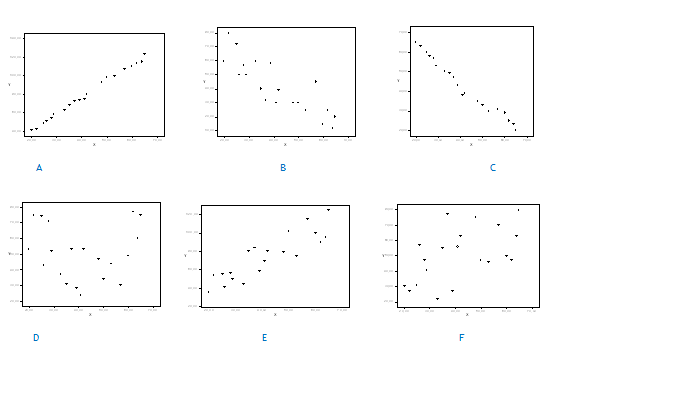
\includegraphics[width=1.10\textwidth]{correlaties.png}
  \captionof{figure}{Correlaties}
  \label{fig:correlaties}
  %\end{figure}
\end{exercise}

\begin{exercise}
  \label{ex:cats}
  Lees het databestand ``Cats.csv'' in. 
  \begin{enumerate}
    \item Voer een lineaire regressieanalyse uit op de variabelen Lichaamsgewicht (\texttt{Bwt}, afhankelijke variabele) en Gewicht hart (\texttt{Hwt}, onafhankelijke variabele).
    \item Maak een spreidingsdiagram van beide variabelen.
    \item Bereken en teken de regressielijn.
    \item Bereken de correlatie- en de determinatiecoëfficiënt.
    \item Geef een interpretatie van deze resultaten.
  \end{enumerate}
\end{exercise}

\begin{exercise}
  \label{ex:cats-per-geslacht}
  Gebruik dezelfde data als in vorige oefening.
  \begin{enumerate}
    \item Voer een lineaire regressieanalyse uit op de variabelen Lichaamsgewicht (Bwt) en Gewicht hart (Hwt) per geslacht.
    \item Maak een spreidingsdiagram van beide variabelen voor elk van de geslachten.
    \item Bereken en teken telkens de regressielijn.
    \item Bereken de correlatie- en de determinatiecoëfficiënt.
    \item Geef een interpretatie aan deze resultaten.
  \end{enumerate}
\end{exercise}

\begin{exercise}
  \label{ex:pizza}
  Lees het databestand ``Pizza.csv'' in.
  \begin{enumerate}
    \item Voer een volledige lineaire regressieanalyse uit op de variabelen Rating en CostPerSlice. Trek hieruit de juiste conclusies en ga deze ook grafisch na.
    \item Onderzoek een mogelijk verband tussen Rating en Neighbourhood. Welke methode kan je hiervoor gebruiken? Kan je de gegevens van Rating hiervoor in dezelfde vorm gebruiken?
    \item Geef een interpretatie aan deze resultaten.
    \item Stel de kruistabel grafisch voor met een staafdiagram.  Voorzie een legende.
  \end{enumerate}
\end{exercise}


%%%%%%%%%%%%%%%%%%%%%%%%%%%%%%%%%%%%%%%%%%%%%%%%%%%%%%



\subsection{Antwoorden op geselecteerde oefeningen}
\label{ssec:analyse-2-variabelen-oplossingen}

\paragraph{Oefening~\ref{ex:muziekwijn-analyse}}

$\chi^2 \approx 18,2792$, Cramér's $V \approx 0,1939$

\paragraph{Oefening~\ref{ex:chisq-survey}}

\begin{enumerate}
  \item \texttt{Exer}/\texttt{Smoke}: $\chi^2 = 5.4885$, $g = 12.59159$, $p = 0.4828422$
  \item \texttt{W.Hnd}/\texttt{Fold}: $\chi^2 = 1.581399$, $g = 5.9915$, $p = 0.454$
  \item \texttt{Sex}/\texttt{Smoke}: $\chi^2 = 3.554$, $g = 7.8147$, $p = 0.314$
  \item \texttt{Sex}/\texttt{W.Hnd}: $\chi^2 = 0.236$, $g = 3.8415$, $p = 0.627$
\end{enumerate}

\paragraph{Oefening~\ref{ex:chisq-aids2}} $\chi^2 = 1083.372914$, $g = 14.067140$, $p \approx 1.157 \times 10^{-229}$

\paragraph{Oefening~\ref{ex:chisq-digimeter}} $\chi^2 \approx 6.6997$ ($df = 6$), $g \approx 12.5916$, $p \approx 0.3495$


\paragraph{Oefening~\ref{oef:casus-akin2016-toets}}

Tabel~\ref{tab:akin2016-resultaten-ttoets} geeft een overzicht met voor elke datasetgrootte het beste en tweede beste persistentietype (op basis van het steekproefgemiddelde). De conclusie van~\textcite{Akin2016}, dat \emph{Realm} het performantste persistentietype is, blijft overeind, maar voor de kleine datasets is het verschil niet significant.

Merk op dat we hier niet expliciet vooraf een significantieniveau gekozen hebben. Voor $\alpha = 0,1$, $0,05$ of zelfs $0,01$, kunnen we echter dezelfde conclusie trekken.

\begin{table}
  \begin{center}
    \begin{tabular}{llll}
      \toprule
      \textbf{Grootte} & \textbf{Beste} & \textbf{2e beste} & \textbf{$p$-waarde} \\ \midrule
      Small            & Realm          & SharedPreferences & 0.1699     \\
      Medium           & Realm          & GreenDAO          & 0.0002506  \\
      Large            & Realm          & SQLite            & 0.0017     \\ \bottomrule
    \end{tabular}
  \end{center}
  \caption{Resultaten $t$-toets voor de beste en 2e beste persistentietype op basis van steekproefgemiddelde~\autocite{Akin2016}.}
  \label{tab:akin2016-resultaten-ttoets}
\end{table}

\paragraph{Oefening~\ref{ex:test-examen}}

\begin{itemize}
  \item $\beta_{0} \approx 0,6333$, $\beta_{1} \approx 0.9667$
  \item $Cov \approx 6,444$, $R \approx 0,9352$, $R^2 \approx 0,8747$
\end{itemize}

\paragraph{Oefening \ref{ex:cats} en \ref{ex:cats-per-geslacht}}

\begin{center}
  \begin{tabular}{lrrrrr}
  	\toprule
    \textbf{Selectie} & \textbf{$\beta_{0}$} & \textbf{$\beta_{1}$} & \textbf{$Cov$} & \textbf{$R$} & \textbf{$R^2$} \\
    \midrule
  	Hele dataset & -0.3511 & 4.0318 & 0.9496 & 0.8041 & 0.6466 \\
  	Female       &  2.9813 & 2.6364 & 0.1979 & 0.5320 & 0.2831 \\
  	Male         & -1.1768 & 4.3098 & 0.9419 & 0.7930 & 0.6289 \\
    \bottomrule
  \end{tabular}
\end{center}

